\chapter{A co-rotational triangular shell FEM model}
\label{chap9}
\begin{shortAbstract}
A short abstract for the upcoming chapter \\
\OC{ISBMS 2010}
\end{shortAbstract}


\section{Model description}

We propose to define a triangular shell element by combining a two-dimensional in-plane membrane energy, with an off-plane energy for describing bending and twist. To allow for real-time simulation, a computationally efficient formulation is needed. We therefore propose to extend the co-rotational idea introduced by \cite{Felippa00}. Indeed, as we have seen in the previous chapters, co-rotational approaches have been successfully applied to real-time simulation over the last few years. They offer a good trade-off between computational efficiency and accuracy by allowing small deformations but large displacements. We propose to improve and extend a plate model first introduced by \cite{Przemieniecki68} to a co-rotational formulation. Once combined with an in-plane membrane formulation we obtain an accurate, yet computationally efficient, shell finite element method featuring both membrane and bending energies. 

\subsection{Triangular elastic membrane}

The computation of the triangular elastic membrane stiffness matrix can be derived from previous works dealing with tetrahedral co-rotational elements \citep[like][for instance]{Muller04}. The element stiffness matrix $\textbf{K}_e$ can be computed as follows:
%
\begin{equation}
\textbf{K}_e = \int_v \textbf{J} \boldsymbol\chi \textbf{J}^{T} dV,
\end{equation}
where $\textbf{J}$ is the strain-displacement matrix and $\boldsymbol\chi$ embodies the material's behaviour. The implant is very stiff and we therefore assume that the local deformations remain limited during the deployment and a linear constitutive law is sufficient. Thus in the simple case of Hooke's law we have:
%
\begin{equation}
\boldsymbol\chi = \frac{E}{12(1-\nu^2)}
\begin{bmatrix}
1 & \nu & 0 \\
\nu & 1 & 0 \\
0 & 0 & \frac{1}{2} (1-\nu)
\end{bmatrix}
\end{equation}

The stiffness matrix in the global frame is eventually obtained using the rotation matrix of the element: $\textbf{K} = \textbf{R} \textbf{K}_e \textbf{R}^{T}$ where $\textbf{R}$ describes the rotation of the (triangular) element with respect to its initial configuration.

\subsection{Triangular plate bending}

\begin{figure}
\centering
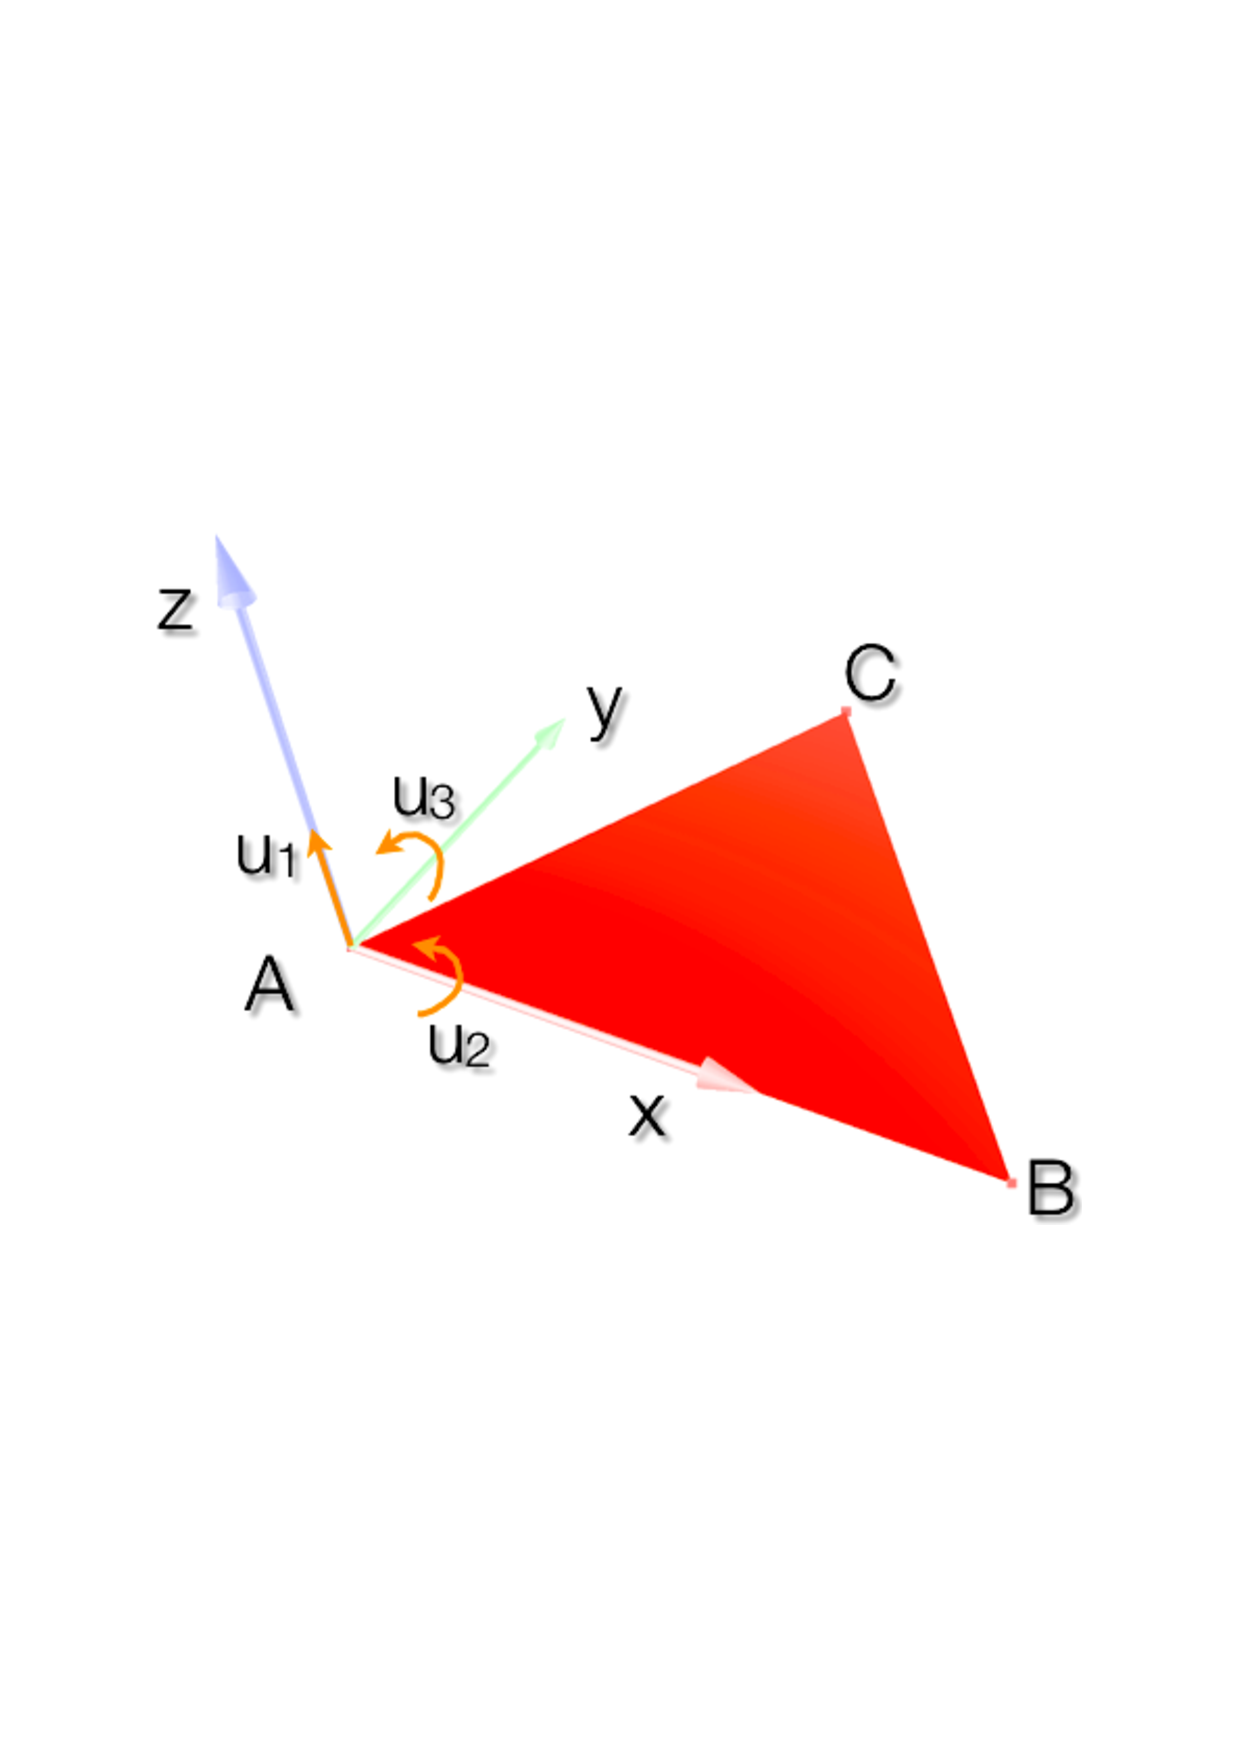
\includegraphics[height=4cm]{chapter9/bending.pdf}
\caption {The different degrees of freedom $u$ of a triangular thin plate in bending.}
\label{chap9:fig-triangle}
\end{figure}
%
To calculate the stiffness matrix for the transverse deflections and rotations shown on \fig{chap9:fig-triangle}, we start with the assumed deflection $u_z$ of the form
\begin{equation}
 u_z = c_1 + c_2x + c_3y + c_4x^2 + c_5xy + c_6y^2 + c_7x^3 + c_8xy^2 + c_9y^3,
\label{chap9:eq-deflection}
\end{equation} 
where $c_1$, \ldots , $c_9$ are constants. Equation~\ref{chap9:eq-deflection} solves an issue of symmetry which was observed with the deflection function proposed by \cite{Przemieniecki68}. These constants can be evaluated in terms of the displacements and slopes at the three corners of the triangular plate using 
\begin{equation}
\textbf{u} = \textbf{Cc}
\label{chap9:eq-U}
\end{equation} 
where $\textbf{u} = \left\{u_1 u_2 \ldots u_9 \right\} $ and $\textbf{c} = \left\{c_1 c_2 \ldots c_9 \right\} $. Matrix $\textbf{C}$ derives from \eqref{chap9:eq-U}:
\begin{equation}
C = 
	\begin{bmatrix}
	1 & 0 & 0 & 0 & 0 & 0 & 0 & 0 & 0 \\
 	0 & 0 & 1 & 0 & 0 & 0 & 0 & 0 & 0 \\
	0 & -1 & 0 & 0 & 0 & 0 & 0 & 0 & 0 \\
	1 & x_2 & 0 & x_2^2 & 0 & 0 & x_2^3 & 0 & 0 \\
	0 & 0 & 1 & 0 & x_2 & 0 & 0 & 0 & 0 \\
	0 & -1 & 0 & -2x_2 & 0 & 0 & -3x_2 & 0 & 0 \\
	1 & x_3 & y_3 & x_3^2 & x_3y_3 & y_3^2 & x_3^2 & x_3y_3^2& y_3^3 \\
	0 & 0 & 1 & 0 & x_3 & 2y_3 & 0 & 2x_3y_3 & 3y_3^2 \\
	0 & -1 & 0 & -2x_3 & -y_3 & 0 & -3x_3^2 & -y_3^2 & 0
	\end{bmatrix}
\end{equation} 

We used the following notations:
\begin{align}
u_1 &= (u_z)_{x_1,y_1}, & u_2 &= \left(\frac{\partial u_z}{\partial y}\right)_{x_1,y_1}, & u_3 &= - \left(\frac{\partial u_z}{\partial x}\right)_{x_1,y_1} \notag \\
u_4 &= (u_z)_{x_2,y_2}, & u_5 &= \left(\frac{\partial u_z}{\partial y}\right)_{x_2,y_2}, & u_6 &= - \left(\frac{\partial u_z}{\partial x}\right)_{x_2,y_2} \label{chap9:ui} \\
u_7 &= (u_z)_{x_3,y_3}, & u_8 &= \left(\frac{\partial u_z}{\partial y}\right)_{x_3,y_3}, & u_9 &= - \left(\frac{\partial u_z}{\partial x}\right)_{x_3,y_3} \notag \\
\end{align} 

\noindent We can calculate the strains from the flat-plate theory using:
\begin{equation}
e_{xx} = -z \frac{\partial^2u_z}{\partial x^2}
\end{equation} 
\begin{equation}
e_{yy} = -z \frac{\partial^2u_z}{\partial y^2}
\end{equation} 
\begin{equation}
e_{xy} = -2z \frac{\partial^2u_z}{\partial x \partial y}
\end{equation} 

\noindent Hence, using the above equations and \eqref{chap9:eq-deflection}, we have
\begin{equation}
\begin{bmatrix}
e_{xx} \\
e_{yy} \\
e_{xy}
\end{bmatrix}
= 
-z
\begin{bmatrix}
0 & 0 & 0 & 2 & 0 & 0 & 6x & 0 & 0 \\
0 & 0 & 0 & 0 & 0 & 2 & 0 & 2x & 6y \\
0 & 0 & 0 & 0 & 2 & 0 & 0 & 4y & 0 \\
\end{bmatrix}
\textbf{c}
\label{chap9:eq-strains}
\end{equation} 
or symbolically $\textbf{e} = \textbf{Dc}$ where $\textbf{D}$ stands for the $3\times 9$ matrix in \eqref{chap9:eq-strains}, including the pre-multiplying constant $-z$. Noting from \eqref{chap9:eq-U} that $\textbf{c} = \textbf{C}^{-1}\textbf{u}$, we have:
\begin{equation}
\textbf{e} = \textbf{DC}^{-1}\textbf{u} = \textbf{bu},
\end{equation} 
where $\textbf{b} = \textbf{DC}^{-1}$. 

\noindent Knowing that the stiffness matrix $\textbf{K}_e$ for an element is obtained from
\begin{equation}
\textbf{K}_e = \int_v \textbf{b}^{T} \boldsymbol\chi \textbf{b} dV,
\end{equation} 
where $\boldsymbol\chi$ is the material matrix, the substitution of $\textbf{b}$ into this expression yields
\begin{equation}
\textbf{K}_e = (\textbf{C}^{-1})^T \int_v \textbf{D}^{T} \boldsymbol\chi \textbf{D} dV \textbf{C}^{-1}.
\end{equation} 
The integration is carried out numerically using Gauss points located at the middle of each edge of the triangle. 

\subsection{Implementation}

In practical terms, the different computations associated with each triangular shell element can be described as follows:
%
\begin{enumerate}
\item Compute the rotation matrix $\textbf{R}$ from global to triangle (local) frame
\item Compute the local displacement vector $\textbf{u} = \{v_1, v_2, 0, u_2, u_3, v_3, v_4, 0, u_5, u_6,$ $v_5, v_6, 0, u_8, u_9 \} $ for each triangle, where $ (v_1, v_2), (v_3, v_4) and (v_5, v_6) $ are the in-plane displacements on x and y local axes and $ u_i $ were defined by \eqref{chap9:ui}. As we are in a co-rotational framework the normal displacements $u_1, u_4, u_7$ at each of the three nodes are null in the local frame of the triangle. 
\item Compute matrix $\textbf{D}_i$  at each Gauss point $i$
\item The strain-displacement matrix at each Gauss point $i$ is computed with $\textbf{J}_i = \textbf{D}_i \textbf{C}^{-1}$
\item Compute the local stiffness matrix $\textbf{K}_e$ of the element as $\textbf{K}_e = \displaystyle{\sum^3_{i=1}} \textbf{J}_i \boldsymbol\chi \textbf{J}_i^T$
\item Transform the local element stiffness matrix into the global frame and add it to a global stiffness matrix
\end{enumerate}

The co-rotational shell formulation has been successfully implemented as a ForceField into the open-source framework SOFA \citep{Allard07}.

\bigskip

\TODO{add a few words about a GPU implementation.}

\section{Validation}

We compared our model with some theoretical results reported by \cite{Zhongnian86} to assess its quality in modelling bending. The test that we carried out uses a square shape mesh clamped on all four edges. A uniform load is then applied on the square and the maximum deflection $z_{max}$ at the centre can be calculated. Several simulations are performed with increasing load values $q$ (ranging from $1$ to $5 N/m^2$) and the following parameters were used: Young's Modulus $E = 1.092 \times 10^6 \,Pa$, Poisson's ratio $\nu = 0.3$, square edge length $L = 10\,m$, thickness $h = 0.1\,m$. Using these particular values it can be shown that $z_{max} = 0.126\,q$. The maximum deflection obtained in our simulations are reported in Table~\ref{chap9:tab-results}. In average we found $z_{max} = 0.1248\,q $, resulting in a $0.93\,\%$ error between our model and theoretical results on that test. 
%
\begin{table}[ht]
	\centering
	\begin{tabular}{p{9cm}|c|c|}
	\cline{2-3}
	\multirow{5}{*}{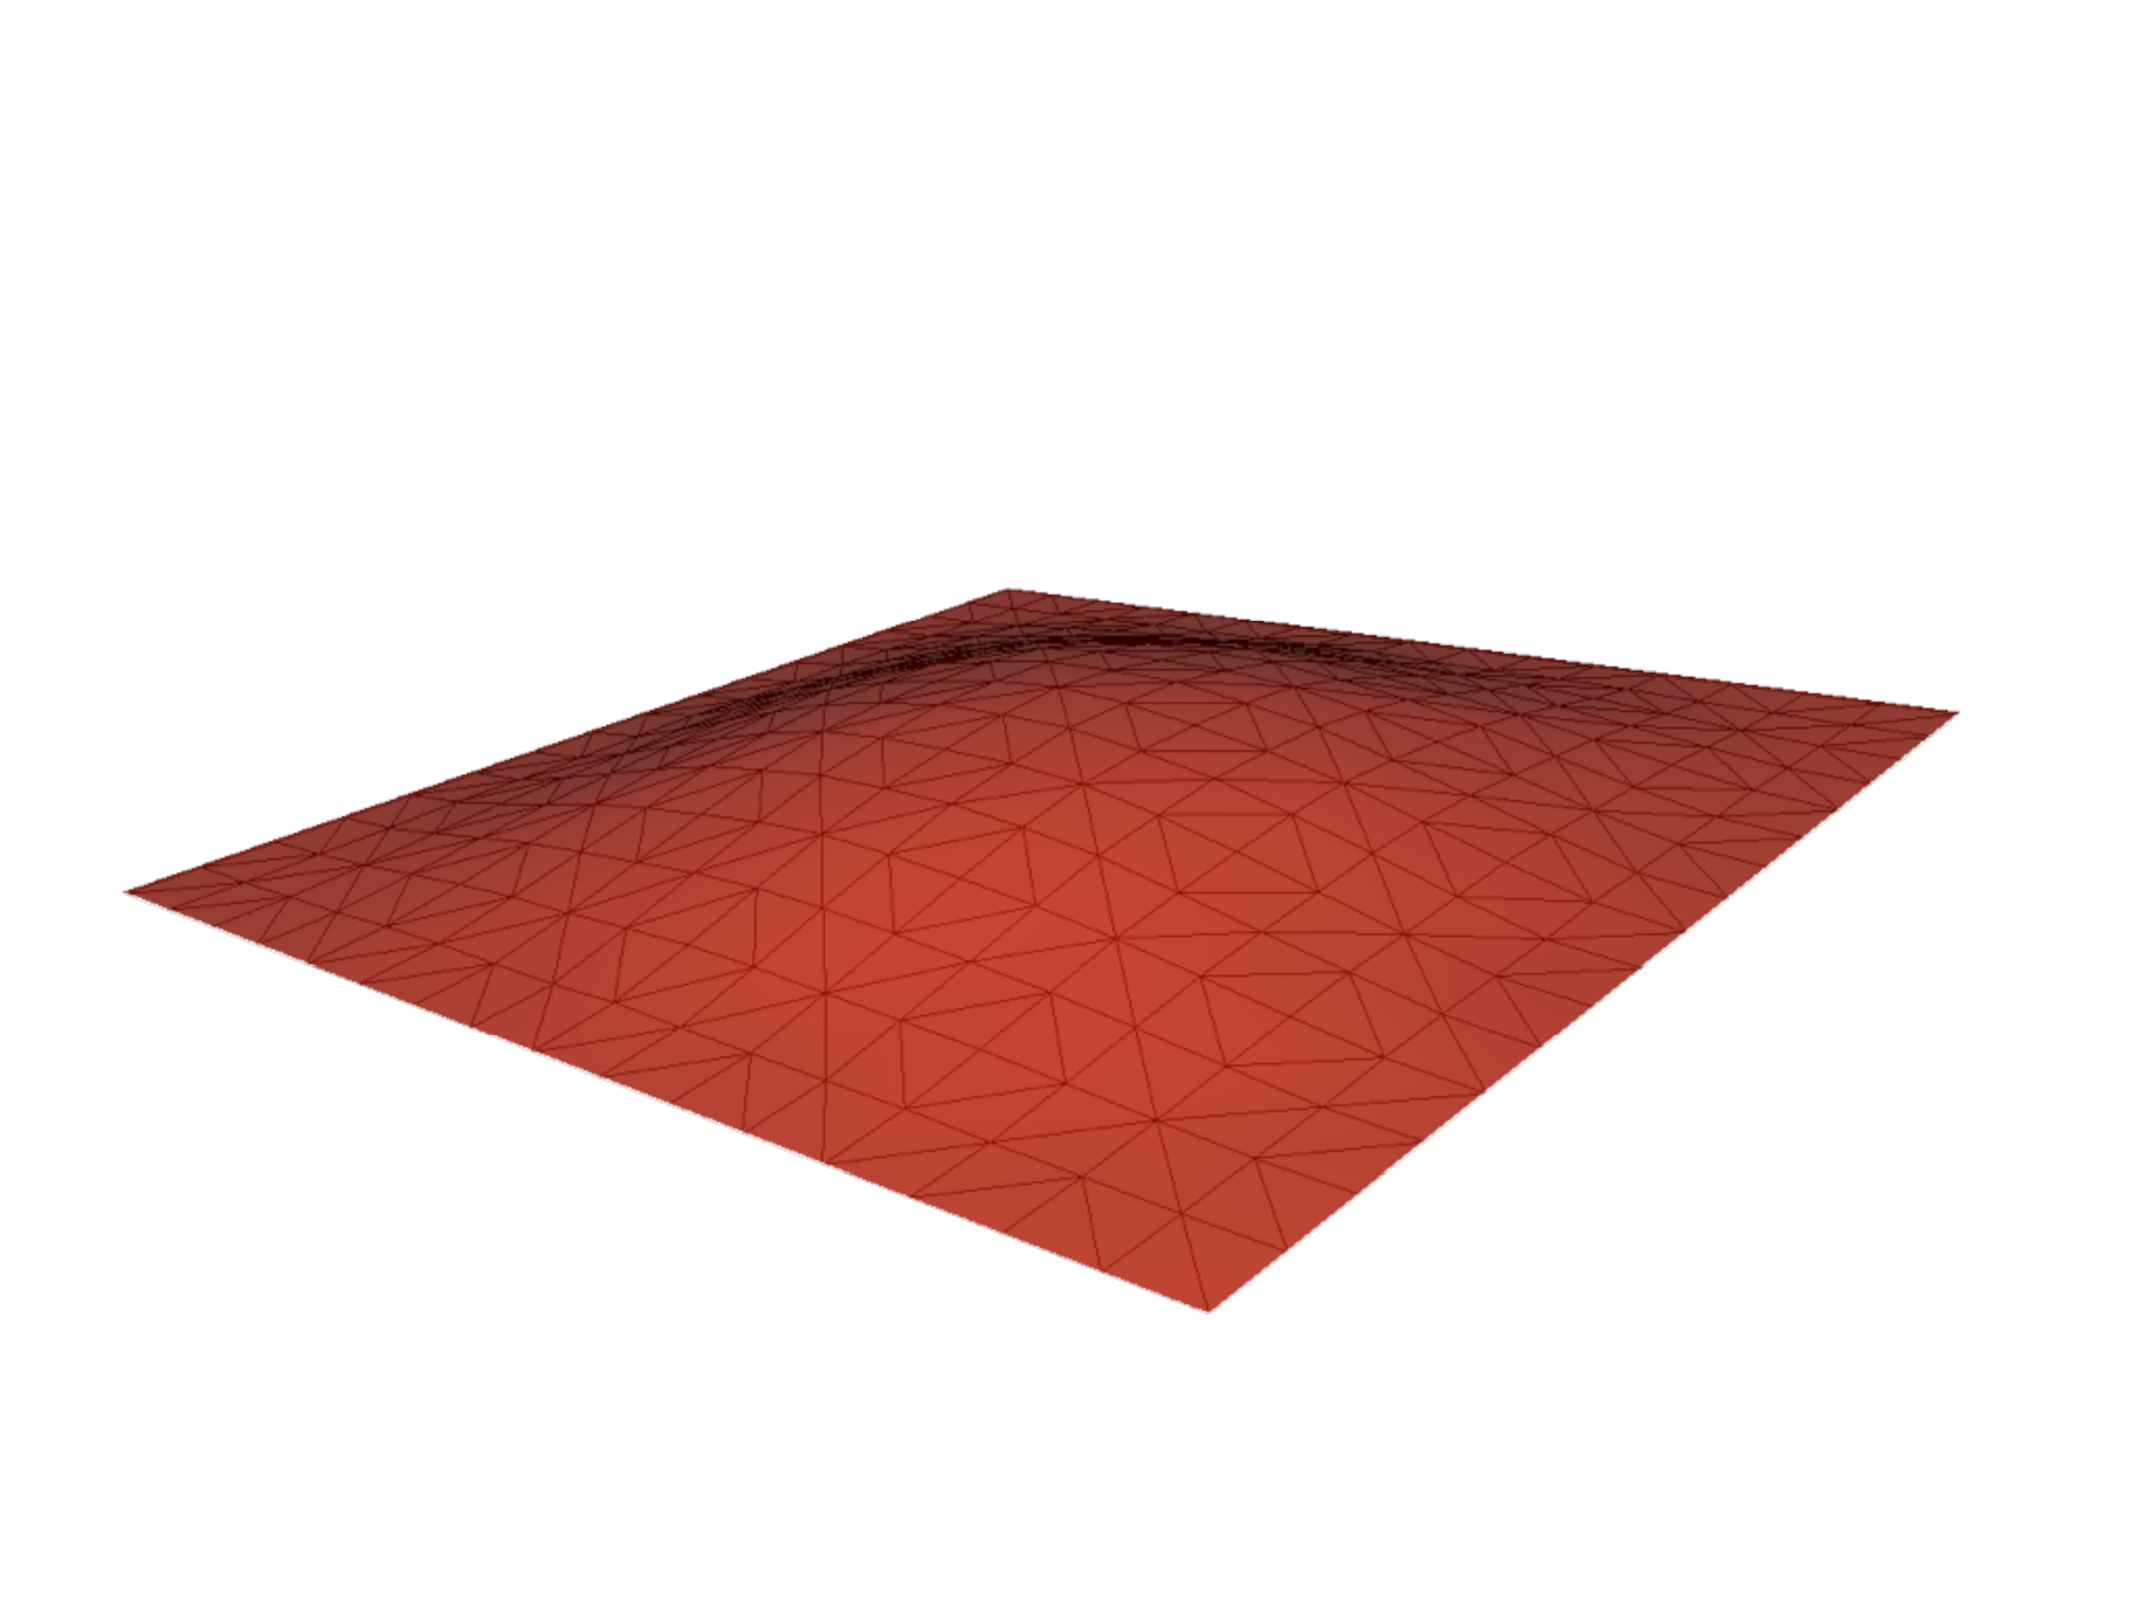
\includegraphics[height=3.5cm]{chapter9/clamped_square.pdf}} & $q$ & $z_{max}$ \tabularnewline
	\cline{2-3}
	& $\,1\,$ & $\, 0.1218 \,$ \tabularnewline
	& $\,2\,$ & $\, 0.2475 \,$ \tabularnewline		
	& $\,3\,$ & $\, 0.3747 \,$ \tabularnewline	
	& $\,4\,$ & $\, 0.5050 \,$ \tabularnewline		
	& $\,5\,$ & $\, 0.6374 \,$ \tabularnewline
	\cline{2-3}
	\end{tabular}
	\vspace{1cm}
	\caption{Comparison of our shell model with theoretical results on the bending of a square plate. An error of less than $1\,\%$ was found between our simulation and theoretical results.}
	\label{chap9:tab-results}
\end{table}


\section{Mechanical interactions with the curved surface of shells}	\label{chap9:interactions}

The practical interest of modelling complex behaviours such as bending and twisting would remain fairly low for medical simulation if contacts and constraints were not handled properly. In our case the difficulty comes from different sources. First the collision detection must be carried out with the curved surface of shell elements as opposed to the classic detection on plane triangles. Then forces applied to a given triangle need to be distributed between linear forces and torques onto its three vertices. As we will see, the same polynomial interpolation function chosen to compute the bending energy in our FEM formulation is also used to capture the interactions between the curved surface and other objects. 

In order to detect the collision with the bent surface, we have chosen the subdivision approach. We first sample the flat surface of each element by recursively dividing each triangle into four smaller ones and the deflection of each new vertex is computed using \eqref{chap9:eq-deflection} according to the displacements and slopes at the three vertices of the triangular element. This process of subdivision allows us to render each shell as a curved triangle (\fig{chap9:fig-shell} (a) and (b)) and detect any collision with the curved surface of the shell using any of the classic collision detection algorithms working on flat triangles.

Once a collision has been detected, it must be processed by distributing the linear force received on the bent surface between the three vertices of the triangle. First the linear part of the force is simply transmitted on each node using the barycentric coordinates of the contact point's projection onto the triangle. 

The main difficulty is to convert the normal component of the force applied to the bent surface into a torque at each of the three nodes (\fig{chap9:fig-shell} (c)). Our approach is the following: during force computation, we use the change in orientation measured at each node to compute the local deflection of each subvertex within the triangle. Differentiating the formulation twice yields a relation between the torque applied at each node and the generated force in bending. We therefore need to invert the latter formulation to convert a bending force into torques at each vertex. We start by retrieving the normal component of the applied force vector $F_{\mathrm{z}}$. We project the application point of the force into the triangle's plane and compute its local coordinates $(x,y)$. We create the polynom $P$ such as 
%
\begin{equation}
P = F_{\mathrm{z}}(1 \hspace{0.2cm} x \hspace{0.2cm} y \hspace{0.2cm} x^2 \hspace{0.2cm} xy \hspace{0.2cm} y^2 \hspace{0.2cm} x^3 \hspace{0.2cm} xy^2 \hspace{0.2cm} y^3)^T. 
\end{equation}
%
The moments at each vertex are then obtained with 
\begin{equation}
\Omega = (\textbf{C}^{-1})^T P.
\end{equation}
%
Thus, we are able to transmit any force coming from interactions with the curved surface of shells to the mechanical vertices used in our FEM formulation. 
%
\begin{figure}
\centering
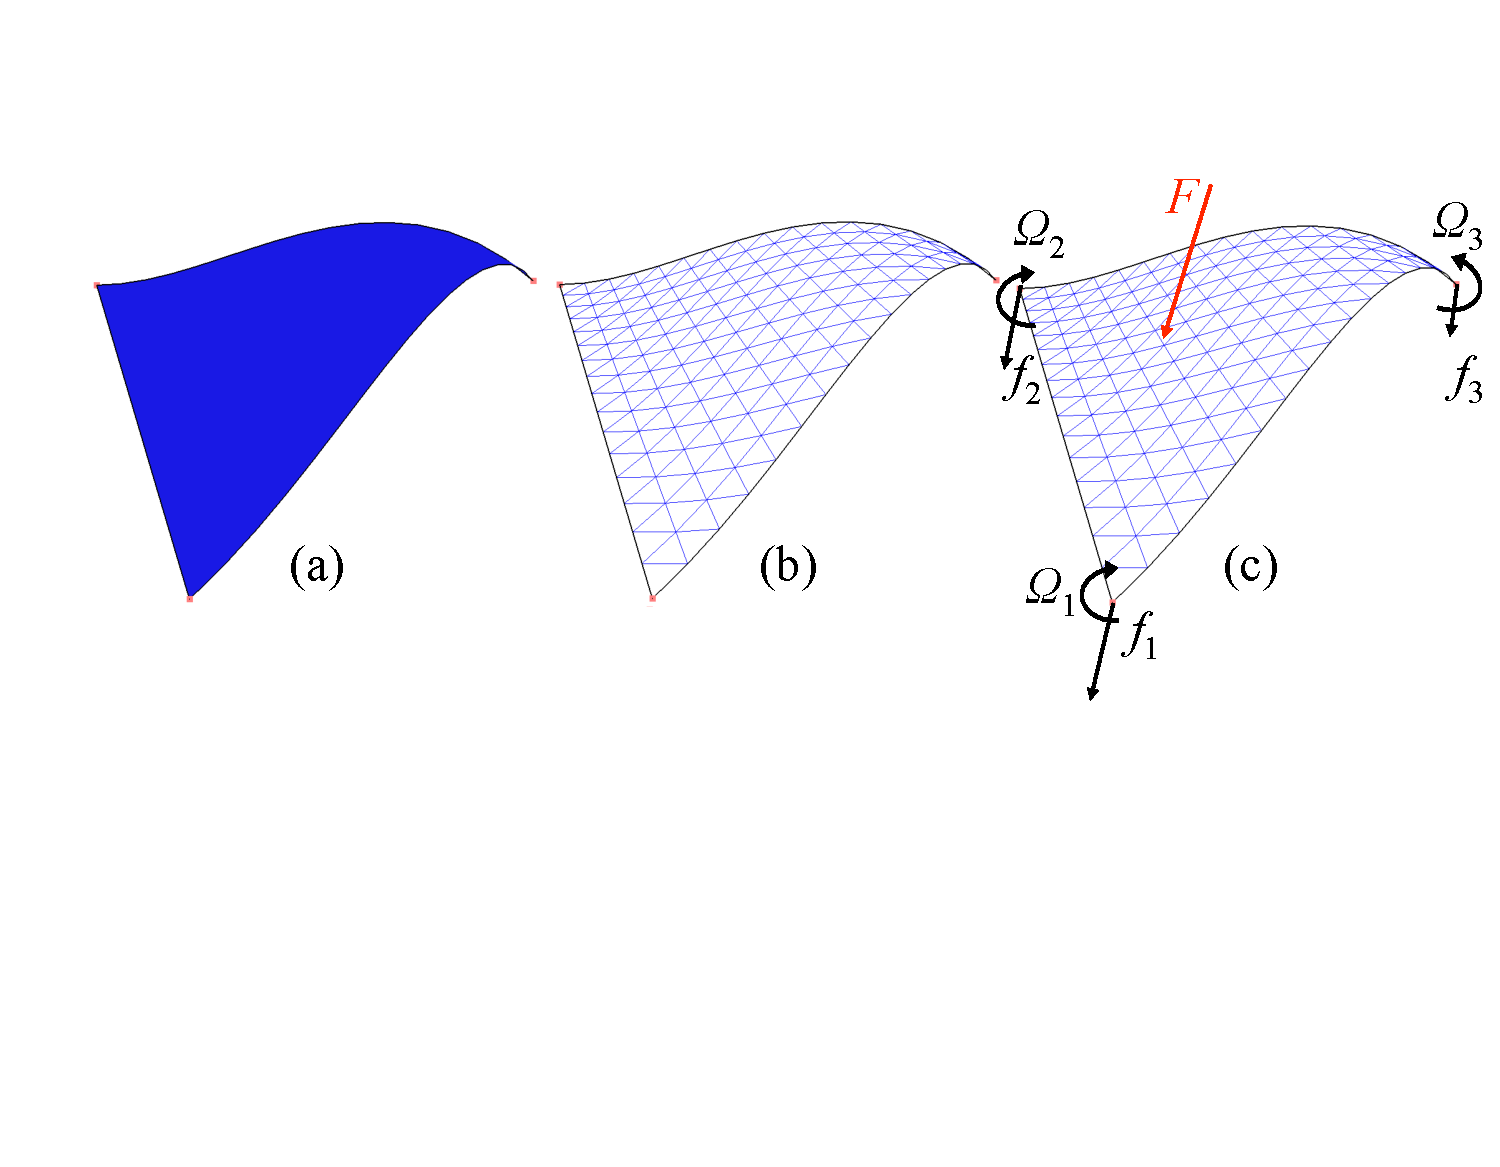
\includegraphics[width=12cm]{chapter9/shell_curvature.pdf}
\caption {(a)  The triangle formed by the three vertices of the shell has been recursively subdivided 3 times and the deflection of each new vertex was computed according to the same deflection function used in our shell FEM. (b) Sampling the actual surface of the shell allows more accurate rendering and collision detection. (c) The shape function is used to distribute an external force $F$ onto the triangle nodes.}
\label{chap9:fig-shell}
\end{figure}


\section{Application to implant deployment simulation in cataract surgery}

Cataract surgery consists in three main steps: capsulorhexis, phacoemulsification, and implantation of an intra-ocular lens. Prior to starting the surgery, a viscoelastic fluid is introduced into the capsule to facilitate capsulorhexis creation and provide protection during phacoemulsification. This fluid remains in the capsule for the duration of the surgery, including the injection of the implant. Capsulorhexis is the technique used to remove a part of the anterior lens capsule. Phacoemulsification consists in using a surgical device which tip vibrates at an ultrasonic frequency to emulsify the natural lens material and then aspirate the  fragments of the cortical material. After the removal of the diseased lens, an intra-ocular lens is implanted into the eye, through a small incision (about 2 mm) using a foldable intra-ocular lens (see \fig{chap9:fig-surgery}). The foldable lens, usually made of acrylic material, is then implanted within the lens capsule through the incision used during phacoemulsification. In some cases the implant can be flipped or  the hooks (also called \emph{haptics}) can break. Therefore the simulation of the insertion and deployment of the implant is crucial for achieving a successful surgery.
%
\begin{figure}[h]
\centering 
\subfloat[ ]{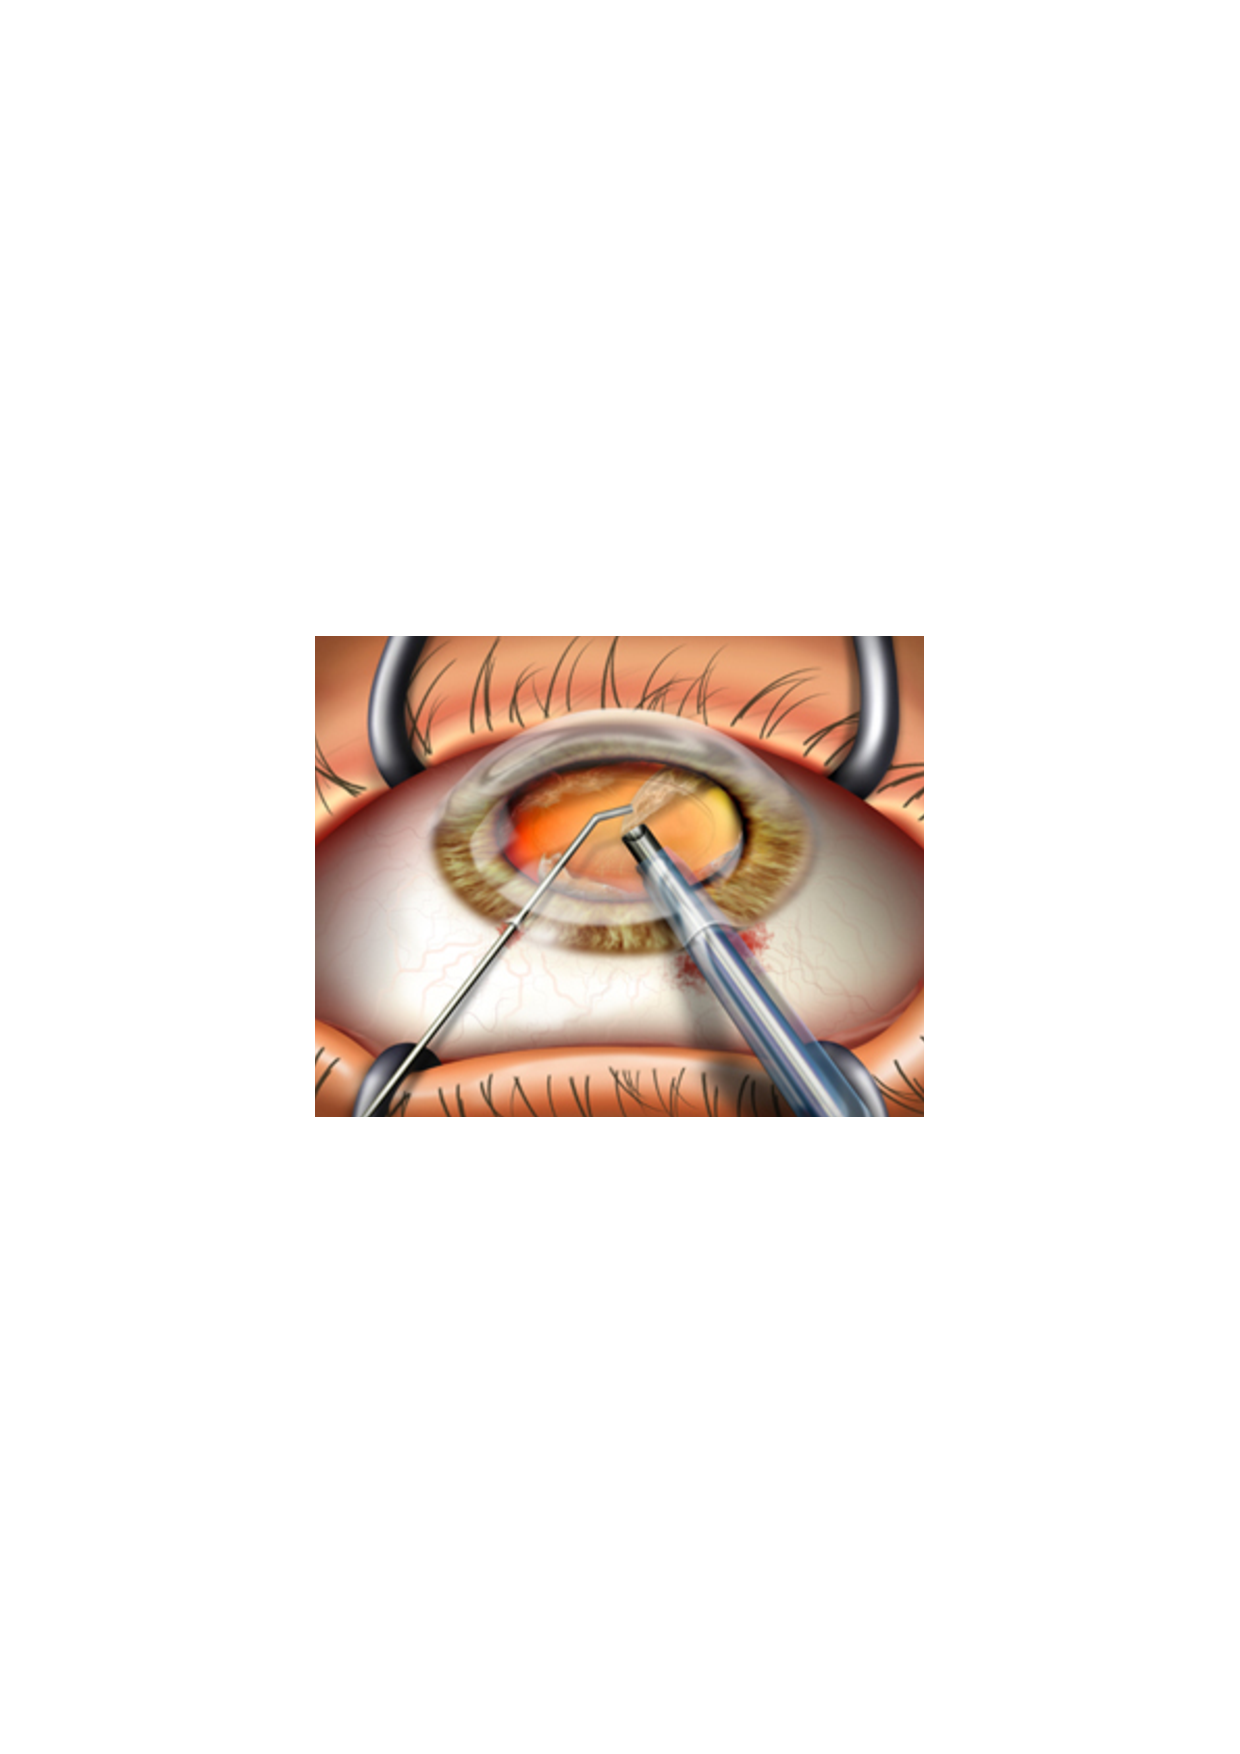
\includegraphics[height=3.2cm]{chapter9/suction.pdf}}
\hspace{1cm} 
\subfloat[ ]{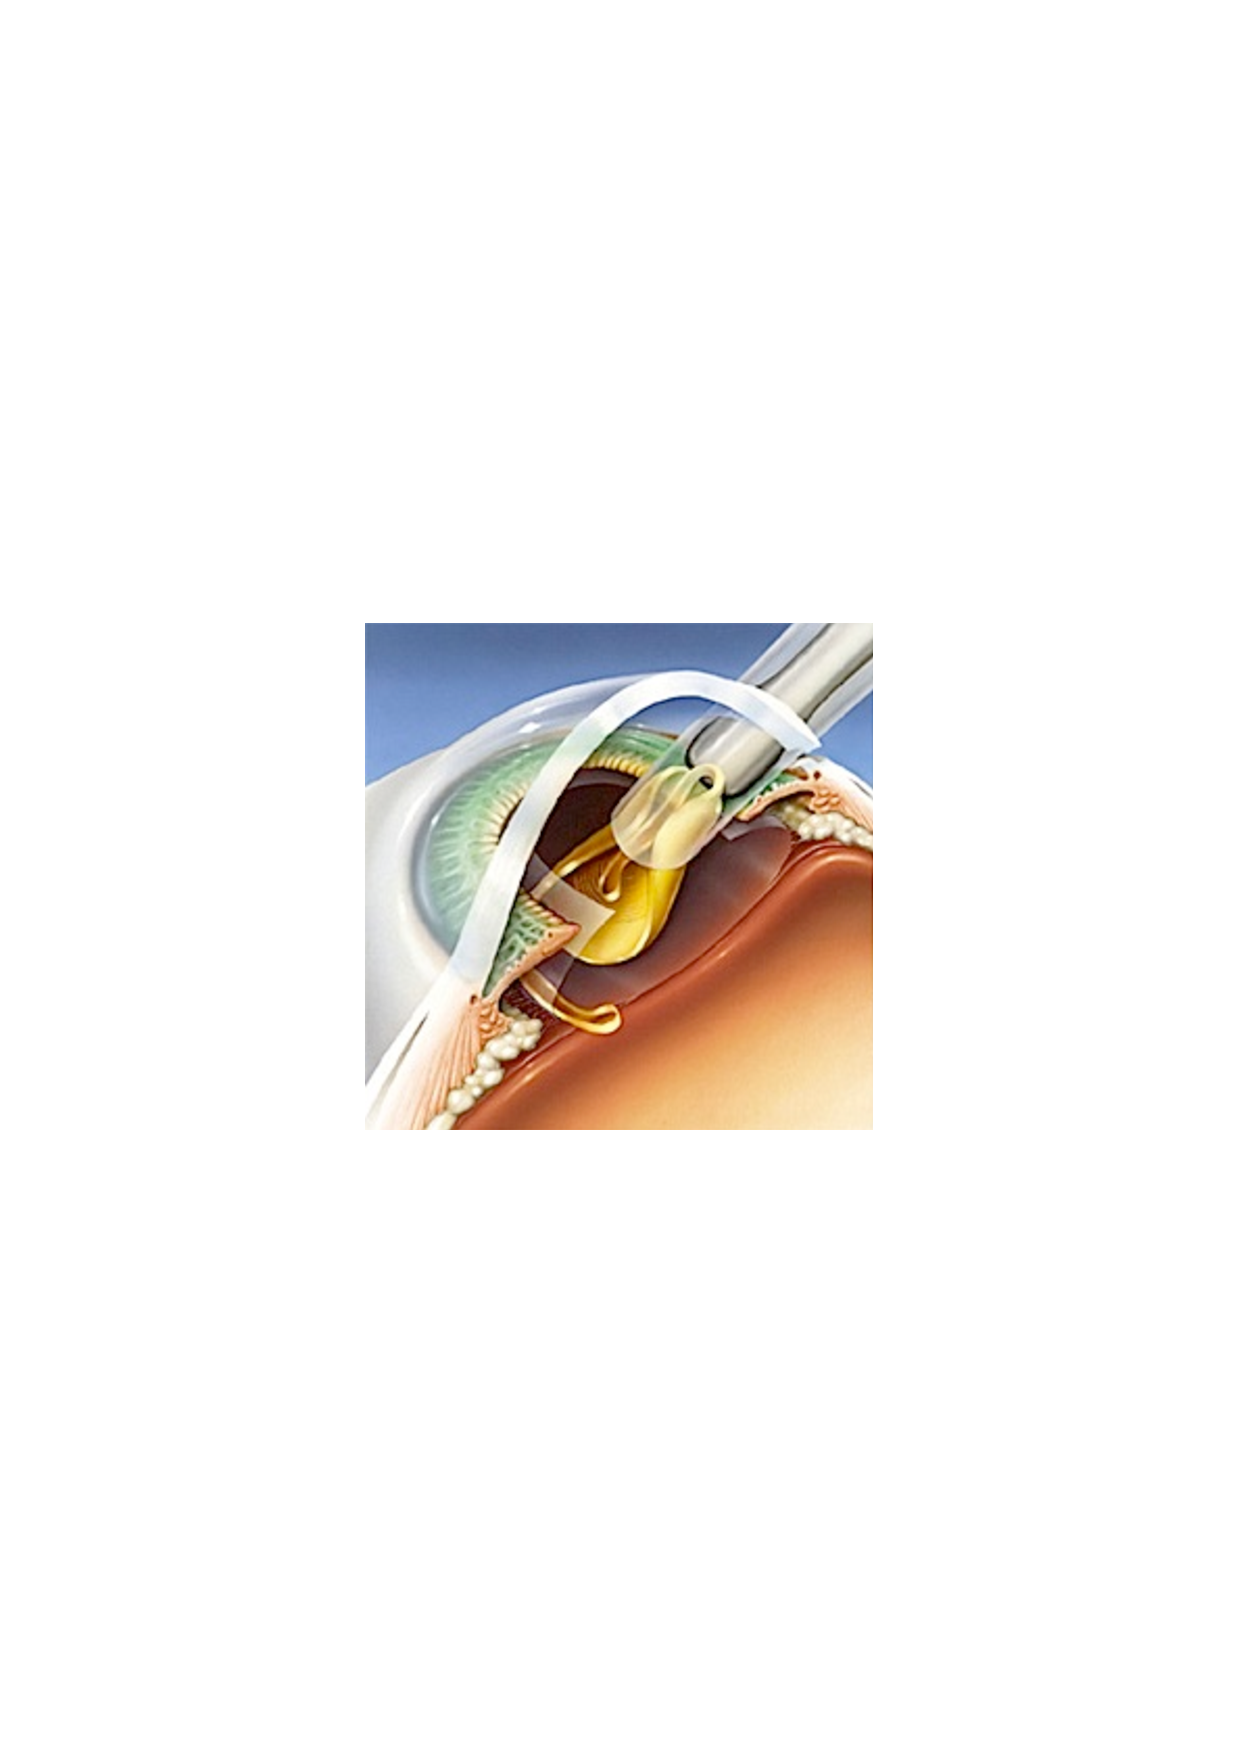
\includegraphics[height=3.2cm]{chapter9/implant_injection_step_1.pdf}}
\hspace{1cm} 
\subfloat[ ]{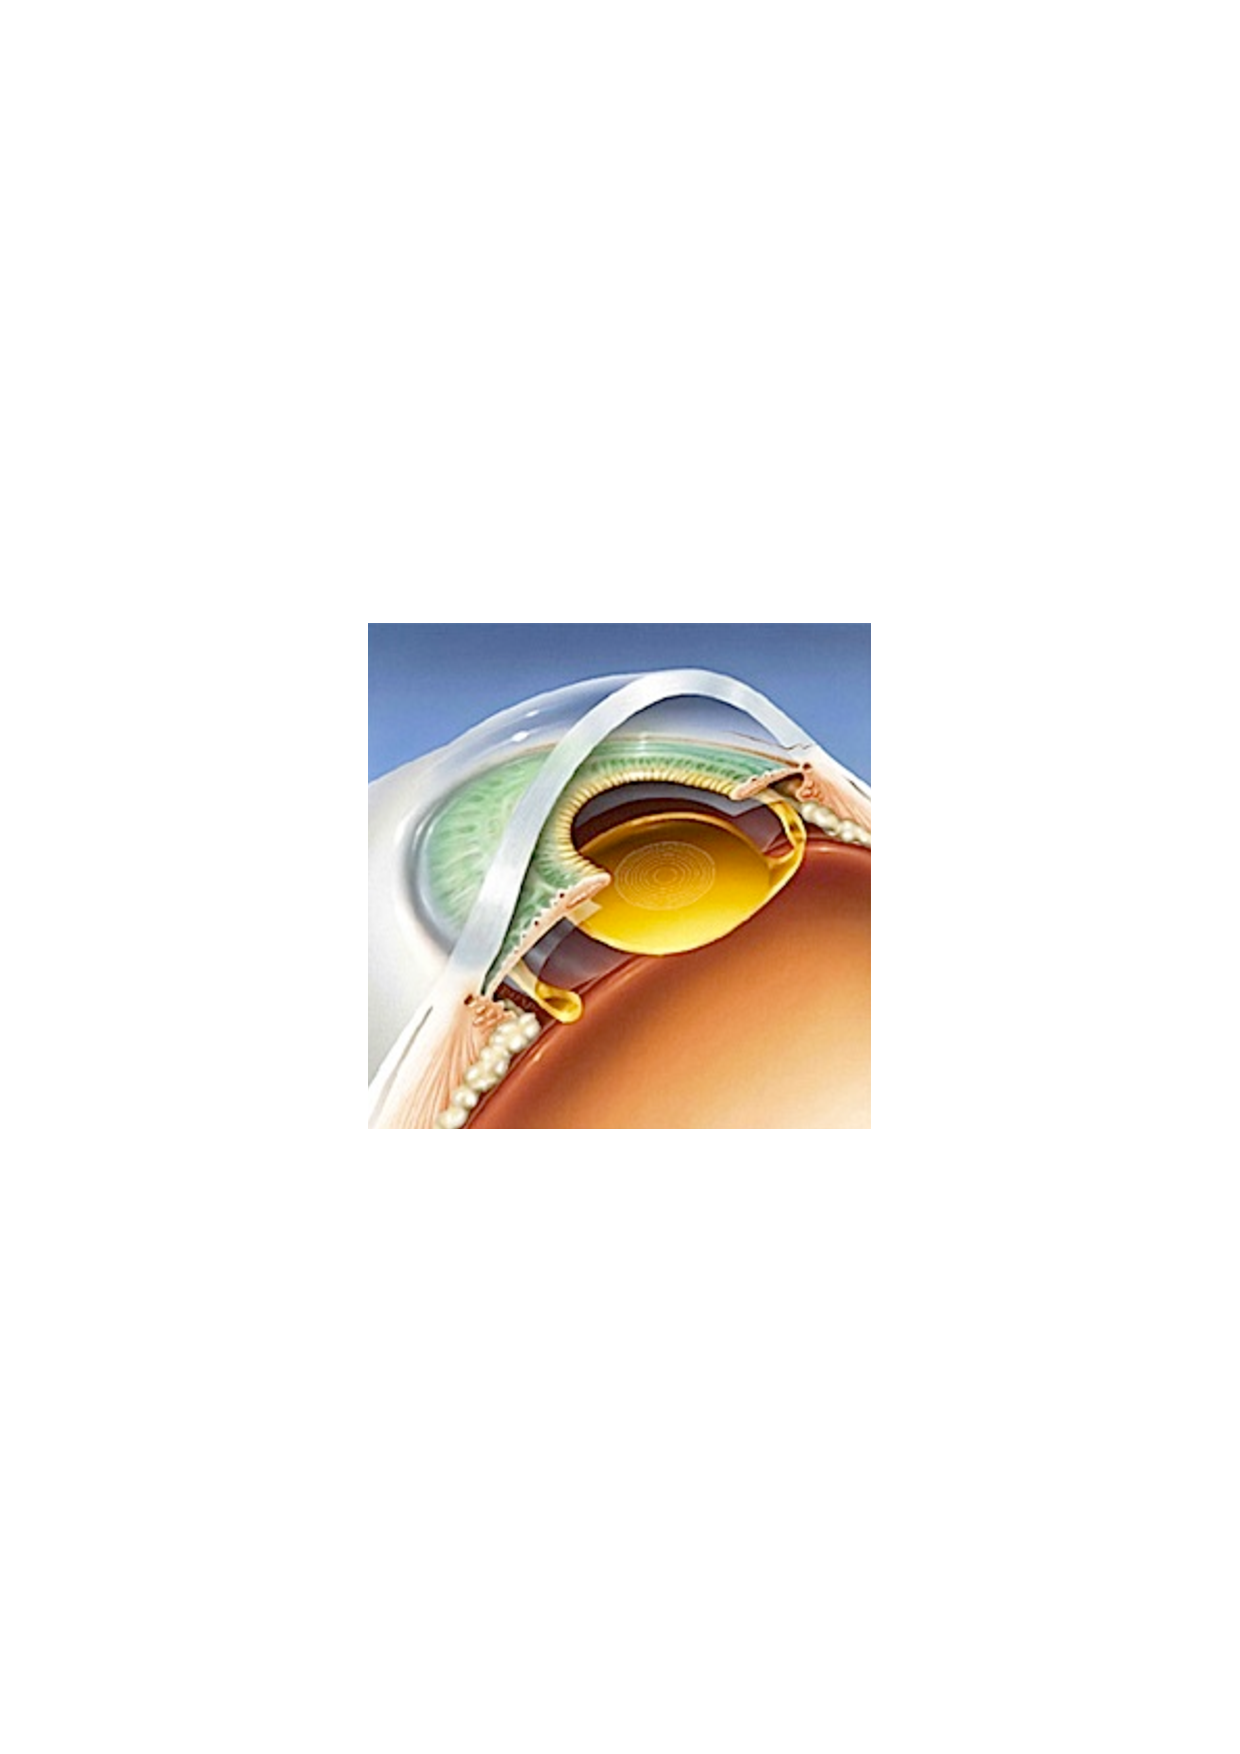
\includegraphics[height=3.2cm]{chapter9/implant_injection_step_2.pdf}}
\caption [Steps of cataract surgery] {(a) removal of the opacified lens by phacoemulsification. (b) insertion of the lens implant which is folded inside the injection device and then deploys within the lens capsule. (c) the lens in place in the capsule.}
\label{chap9:fig-surgery}
\end{figure}

To simulate the insertion and deployment of an intra-ocular lens, we first created a triangulation of the lens surface. Particular care was given to the mesh, to ensure that areas where large stresses occur contain a higher density of elements (see \fig{chap9:fig-mesh}). This was done by noting the constraints applied by the surgeon to the haptics while inserting the implant within the injection device. During this stage, the haptics are folded onto the implant body, leading to high stresses at the junctions. The lens mesh contains $743$ triangles and $473$ nodes. Models of the injection device and the entire eye anatomy were also created. Physical parameters of the lens implant have been provided by the manufacturer Alcon and they are presented in Table~\ref{chap9:tab-parameters}.
%
\begin{table}[h!]
	\begin{center}
		\begin{tabular}{|p{3cm}|p{3cm}|p{3cm}|}
		\hline
		 \centering Young's modulus & \centering Poisson's ratio & \centering Mass density \tabularnewline
		\hline
		\centering $1 MPa$ & \centering $0.42$ & \centering $1.2 g/cm^3$ \tabularnewline
		\hline
		\end{tabular}
	\vspace{0.3cm}
	\caption{Physical parameters of the intra-ocular implant (source: Alcon)}
	\label{chap9:tab-parameters}
	\end{center}
\end{table}

The first difficulty is to obtain the folded geometry of the lens within the injection device. This step is not important for the training process and does not need to be interactive. Indeed the surgeon does not always have to prepare the implant as some injection devices are readily available with a folded implant already in place. We simulate the folding process by first folding the haptics onto the implant body. The body was then bent while keeping the haptics inside to obtain the shape described in \fig{chap9:fig-implantFolding}. The whole process was carried out by applying the necessary forces and boundary conditions on the body and haptics of the implant. The folded implant was then placed into the injection device. The simulation of the injection consists in pushing the intra-ocular implant within the injection device into the lens capsule. During these stages of the simulation, complex contacts occur and consist of self collisions of the lens as well as collisions between the lens and the injector and later with the capsule. To solve the contacts we use the contact warping method proposed by \cite{Saupin08} as it offers an efficient way to compute physically correct contact responses in the case of co-rotational models \TODO{is it still true?}. As adhesions between the haptics and the body is often observed in surgery, friction is also taken into account in the contact response process.
%
\begin{figure}[h]
\centering 
\subfloat[Real implant]{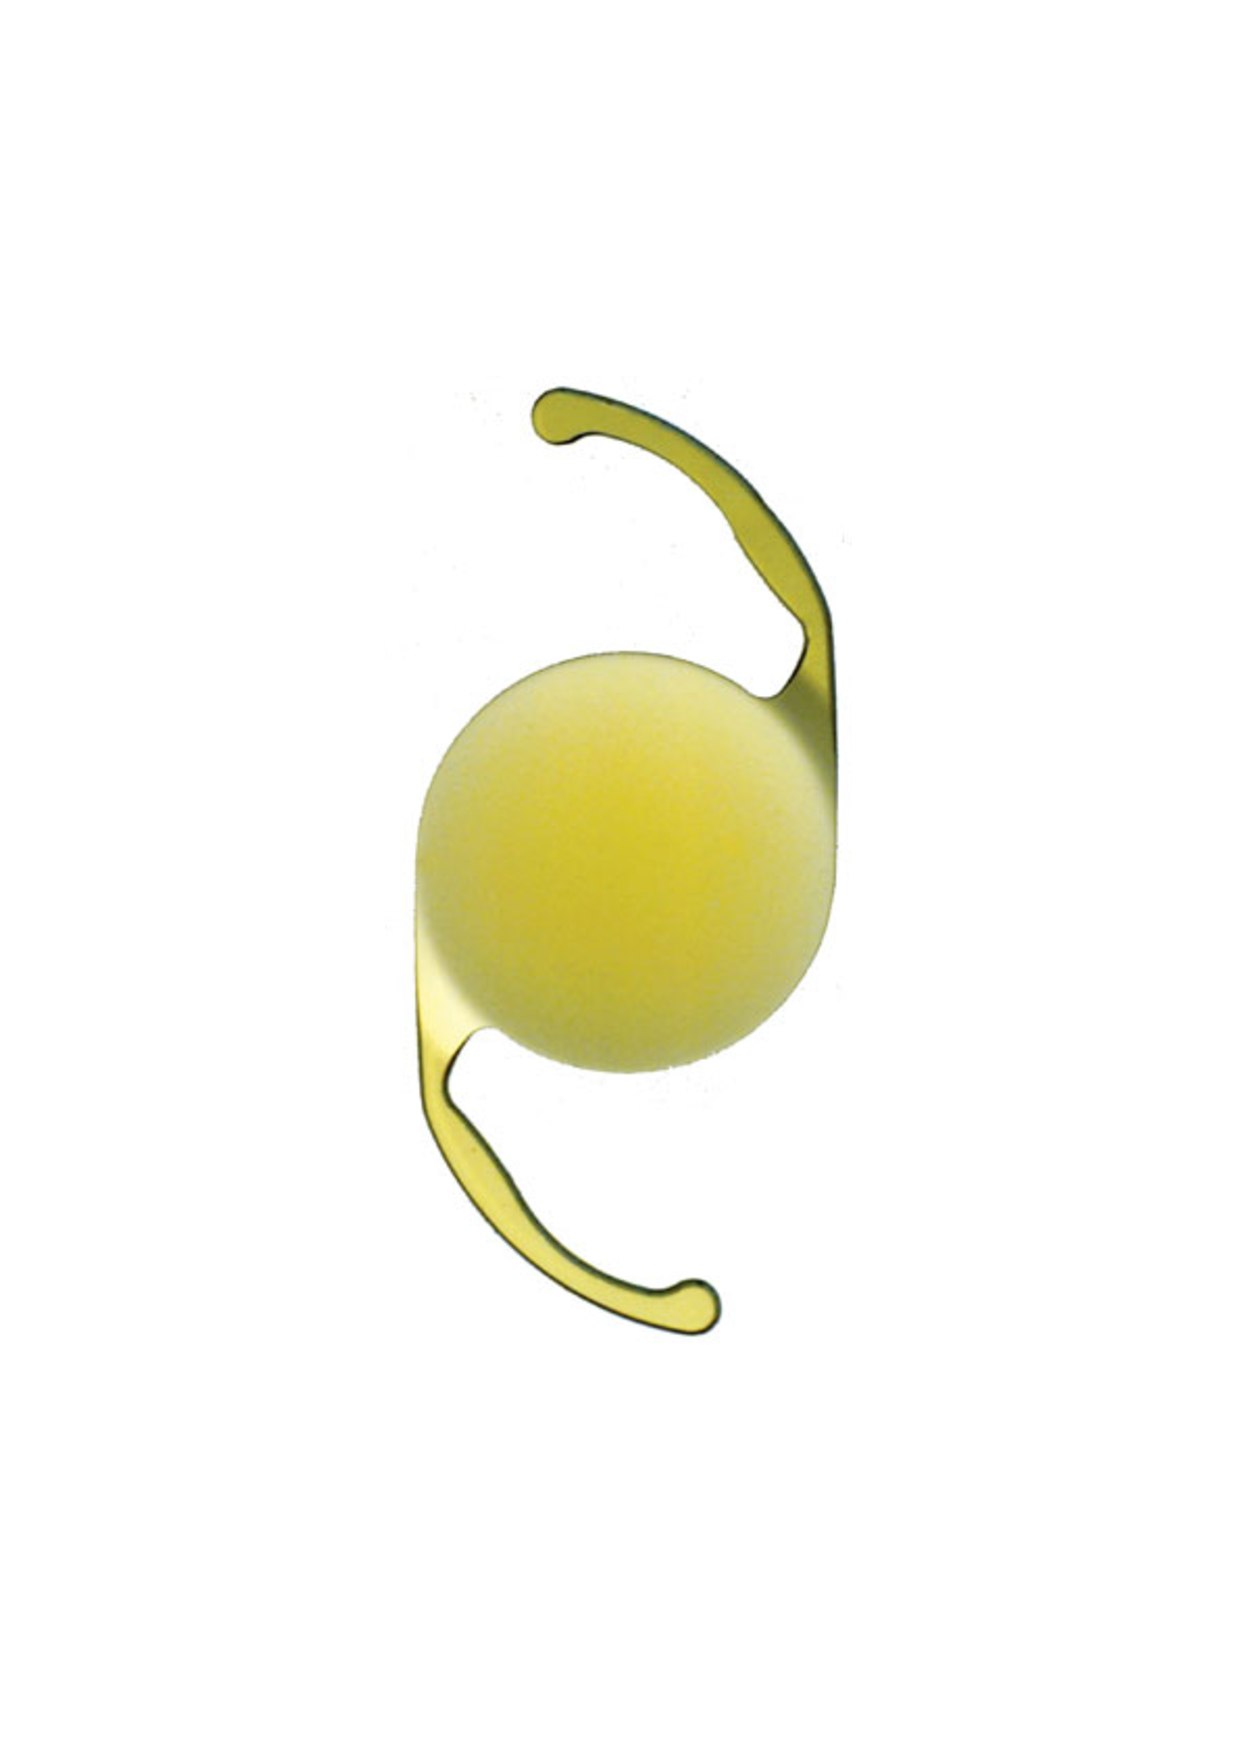
\includegraphics[height=5cm]{chapter9/IOL.pdf}}
\hspace{1cm} 
\subfloat[Meshed model]{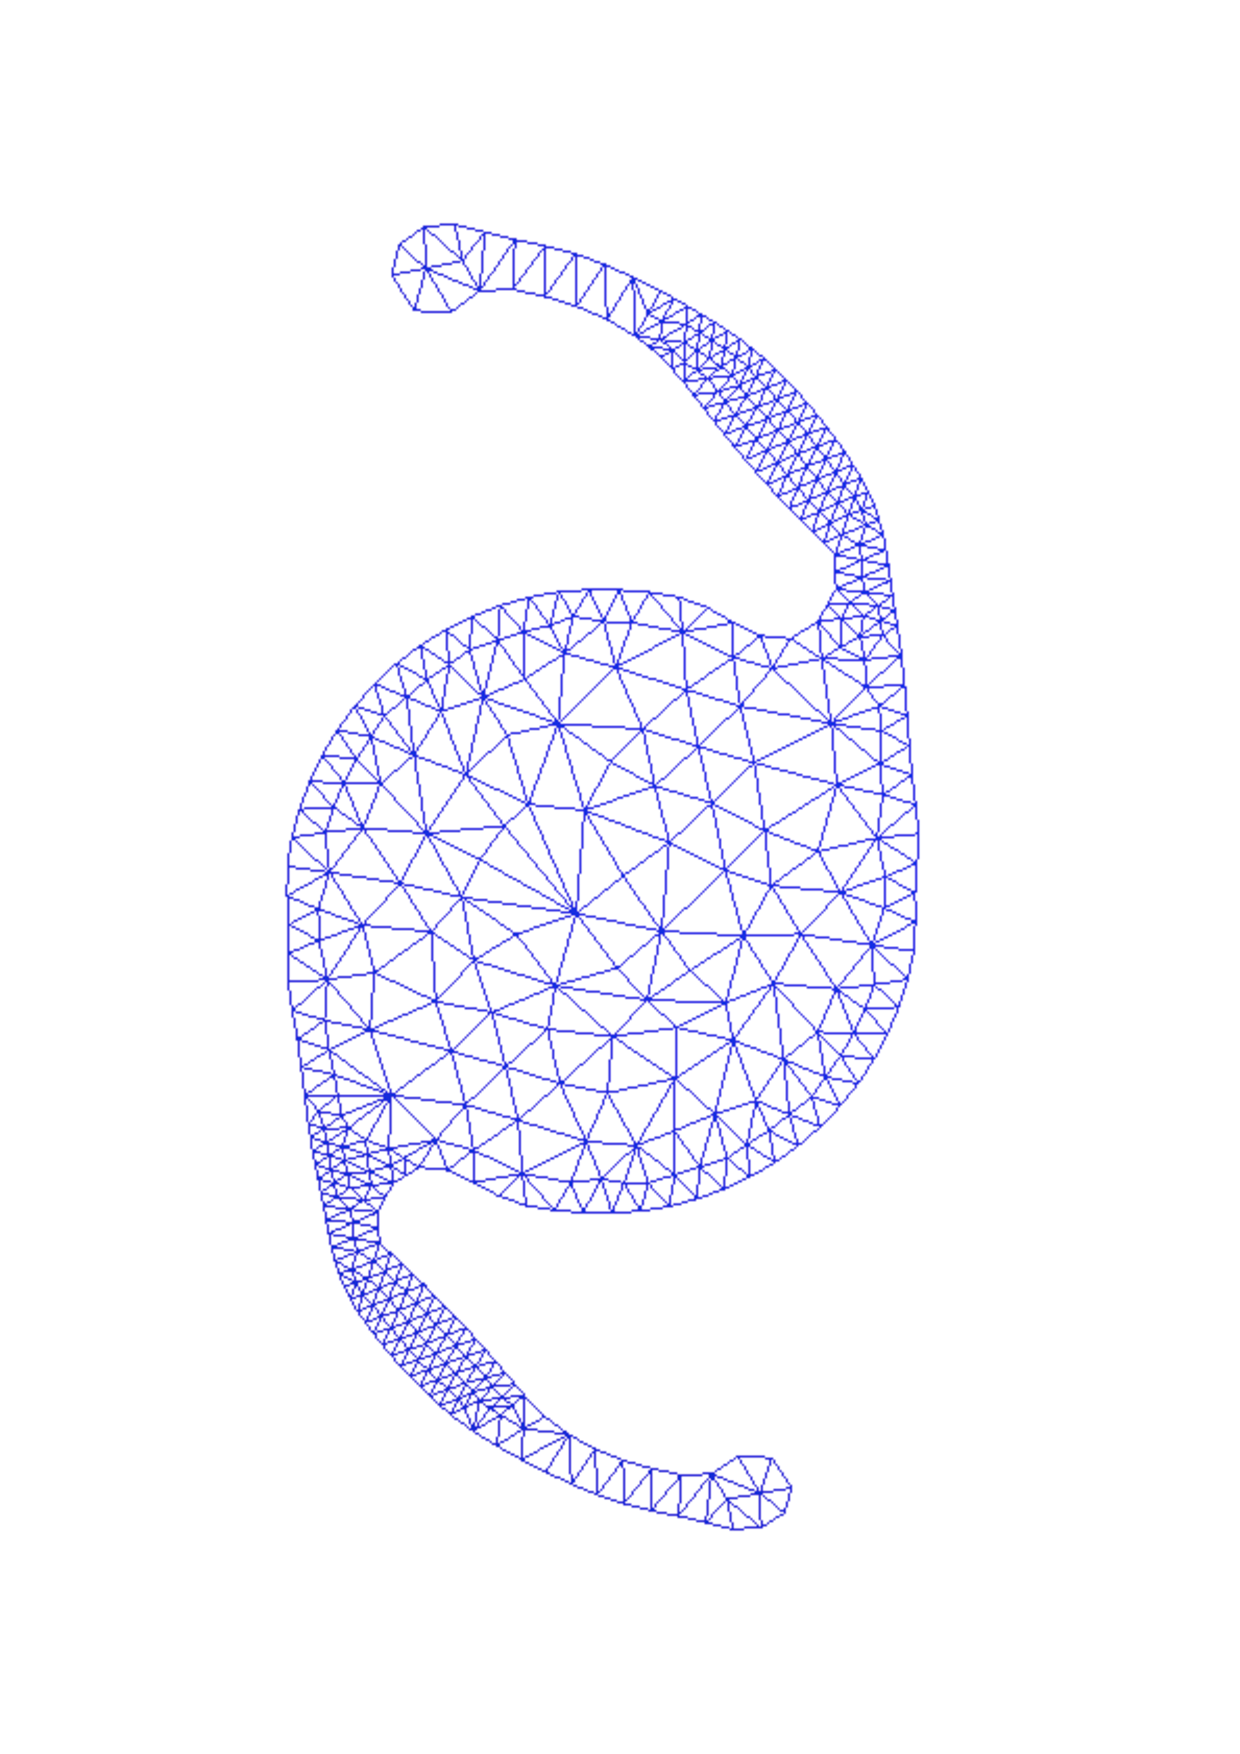
\includegraphics[height=5cm]{chapter9/mesh_implant.pdf}}
\caption [Lens implant and its mesh] {An actual intra-ocular implant (a) and the triangular (b) mesh used in our simulations. Notice the higher density of elements in areas where large deformations will take place. Image of implant courtesy of Alcon.}
\label{chap9:fig-mesh}
\end{figure}

\begin{figure}[!h]
\centering
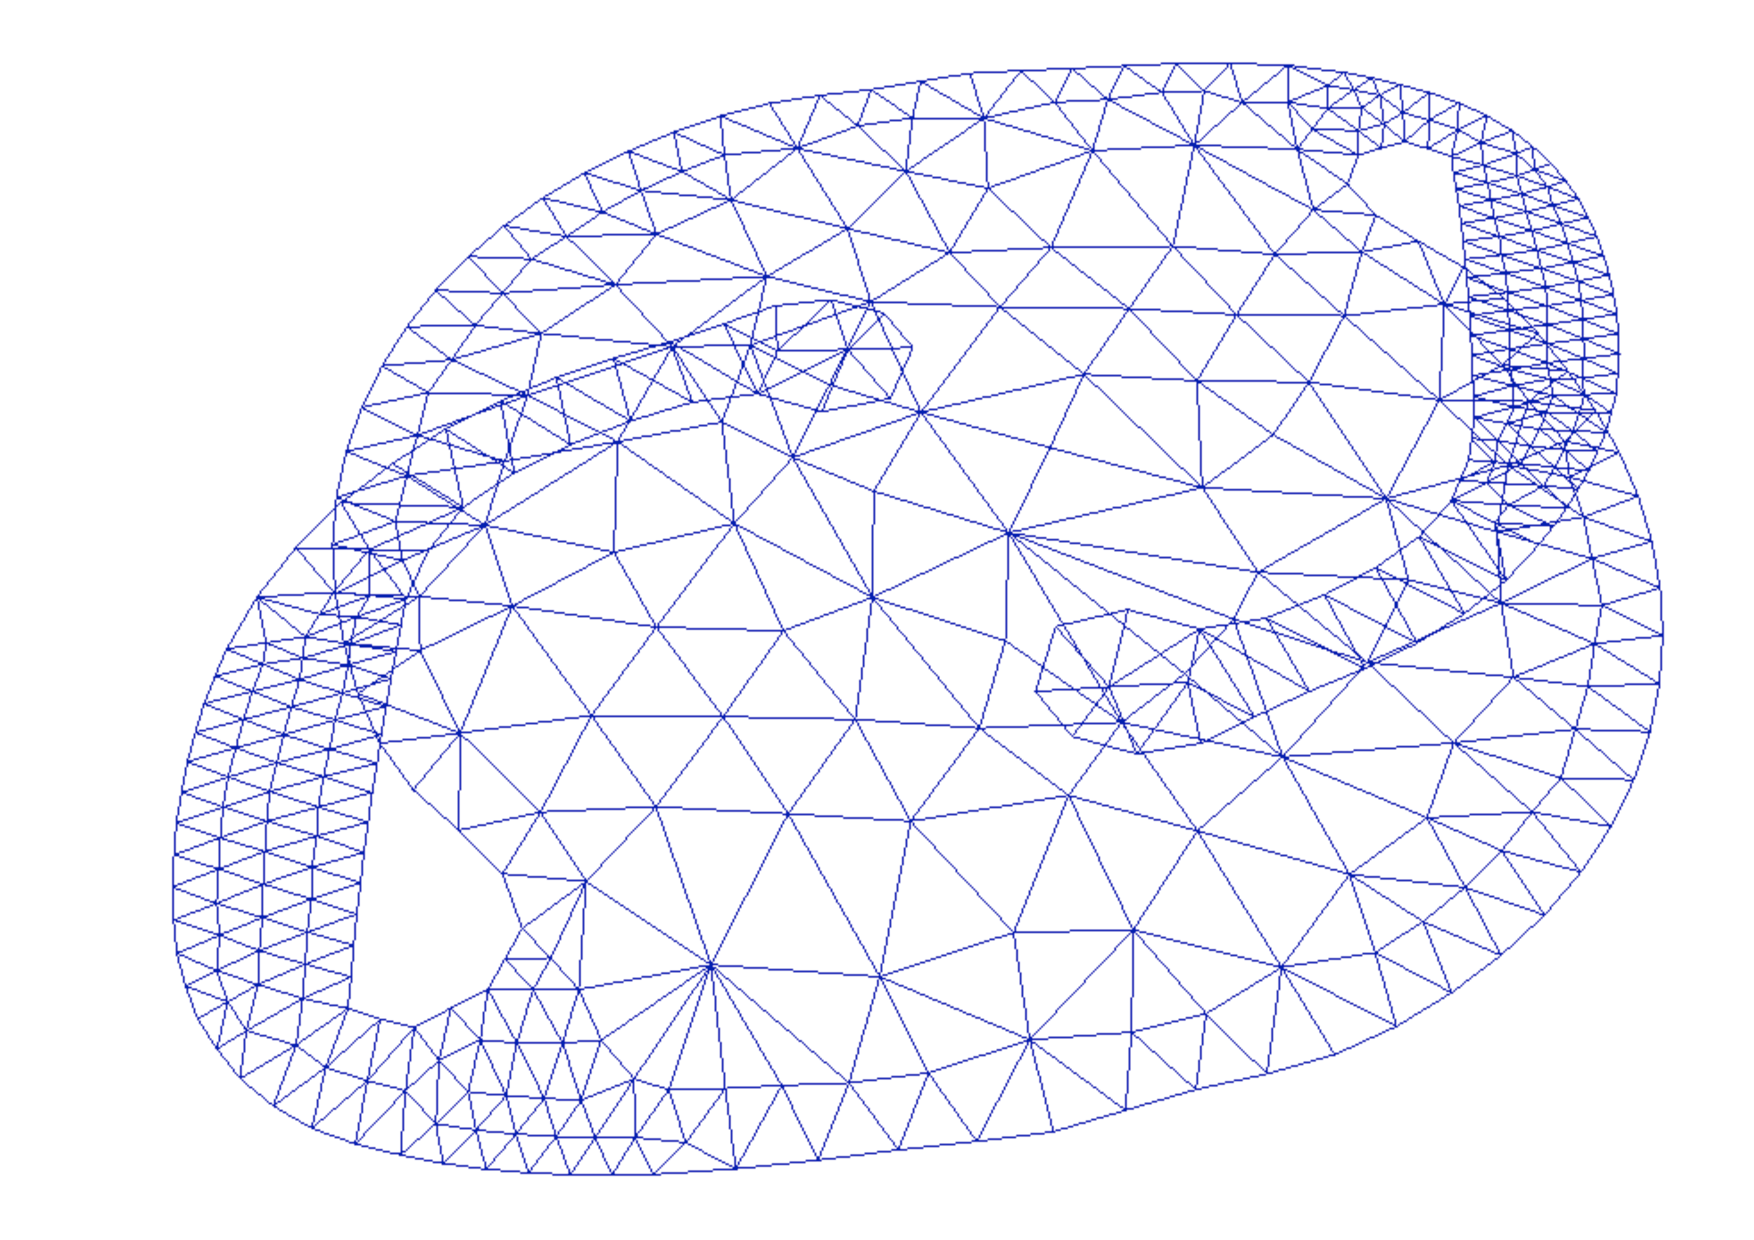
\includegraphics[width=6cm]{chapter9/implant_folding1.pdf}
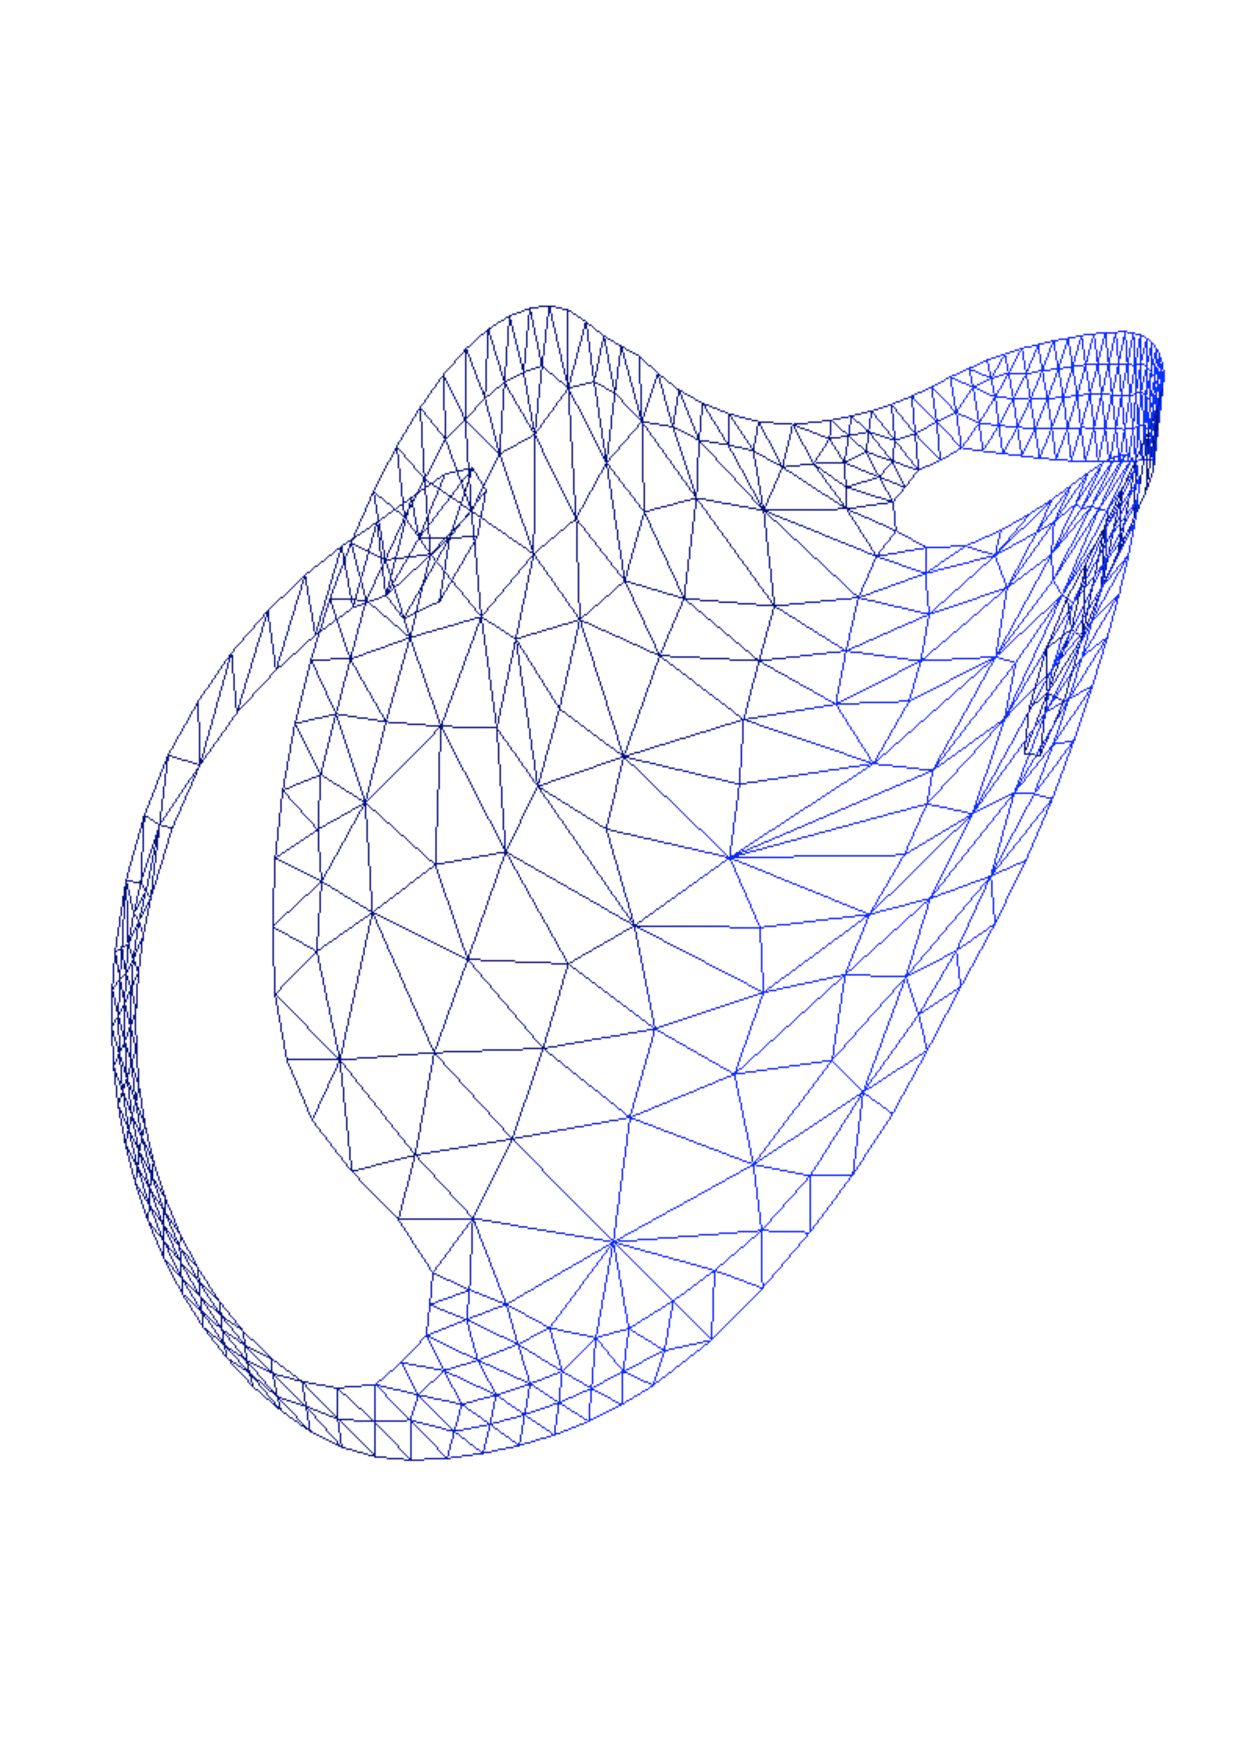
\includegraphics[width=5cm]{chapter9/implant_folding2.pdf} \\
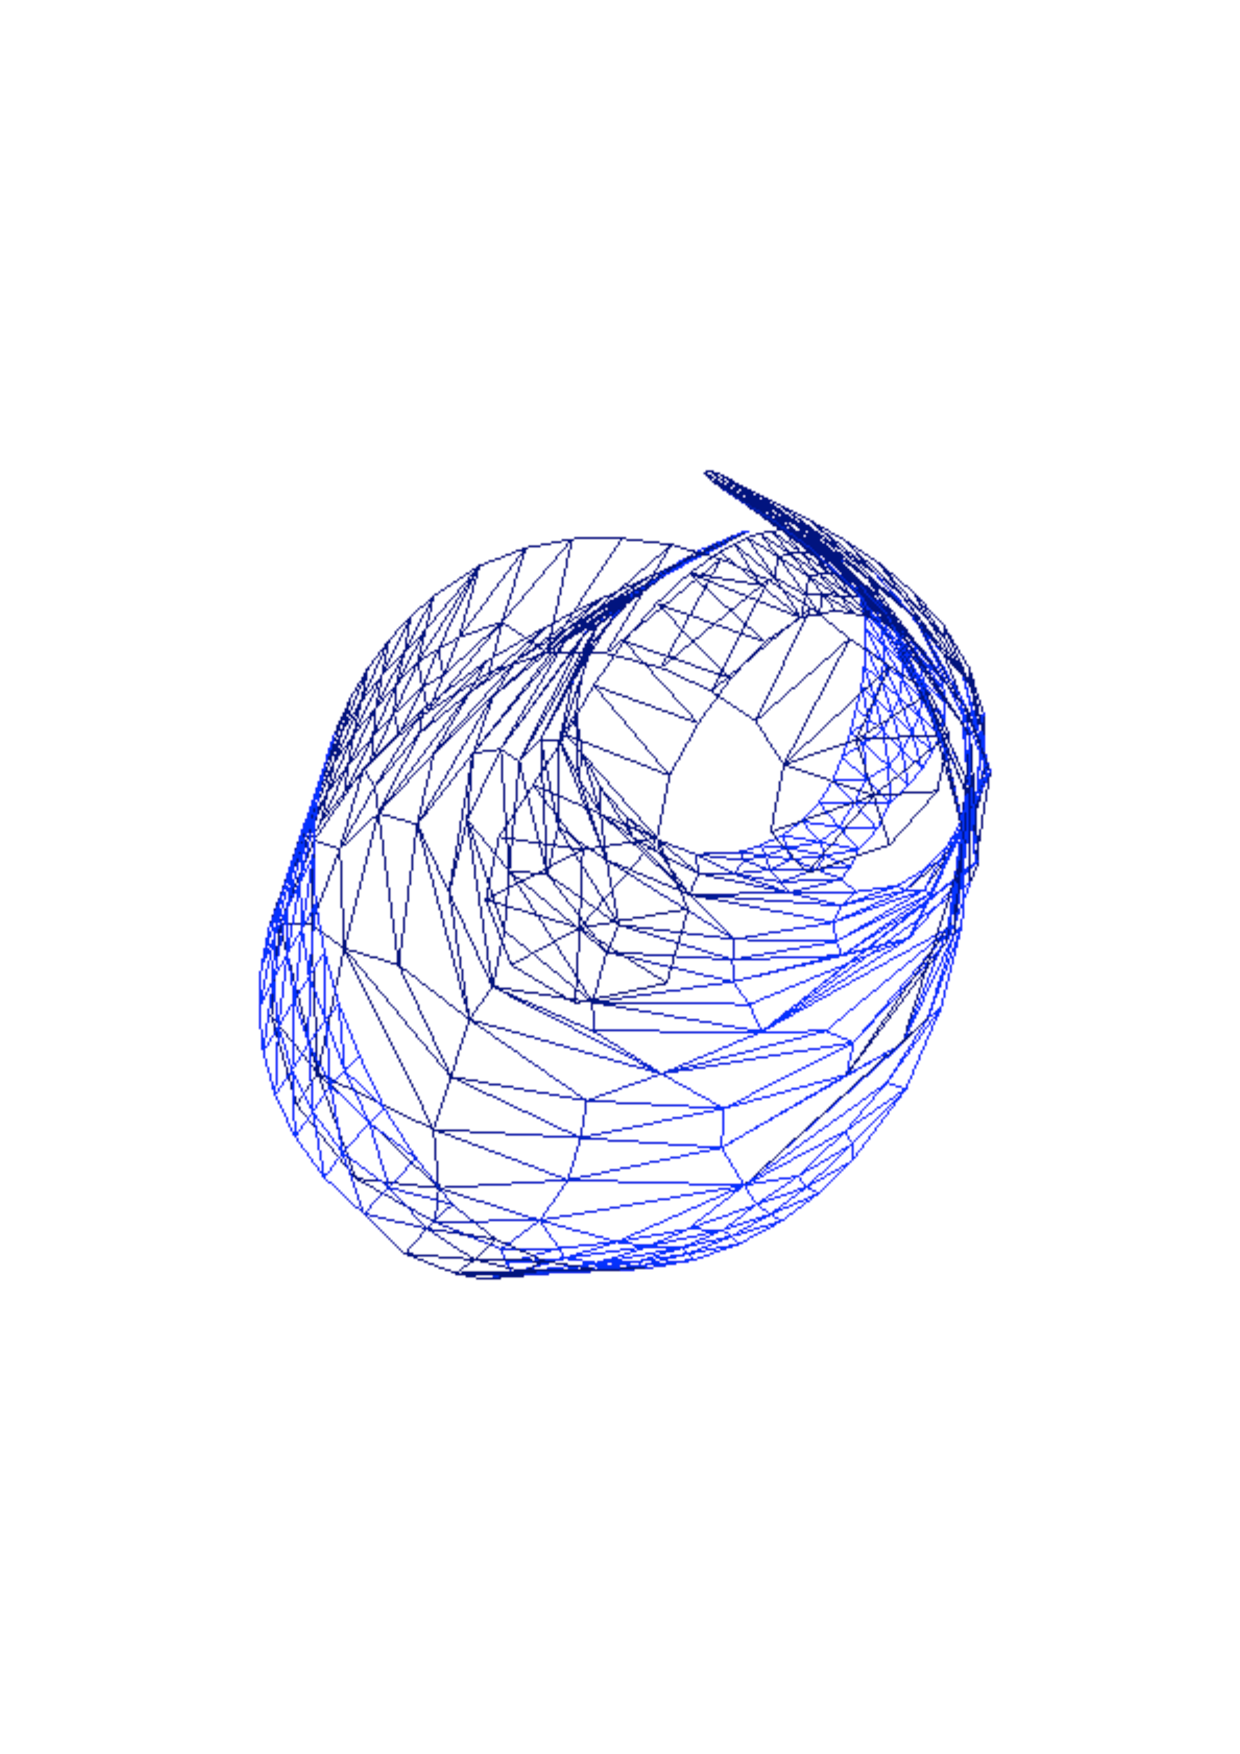
\includegraphics[width=4.5cm]{chapter9/implant_folding3.pdf}
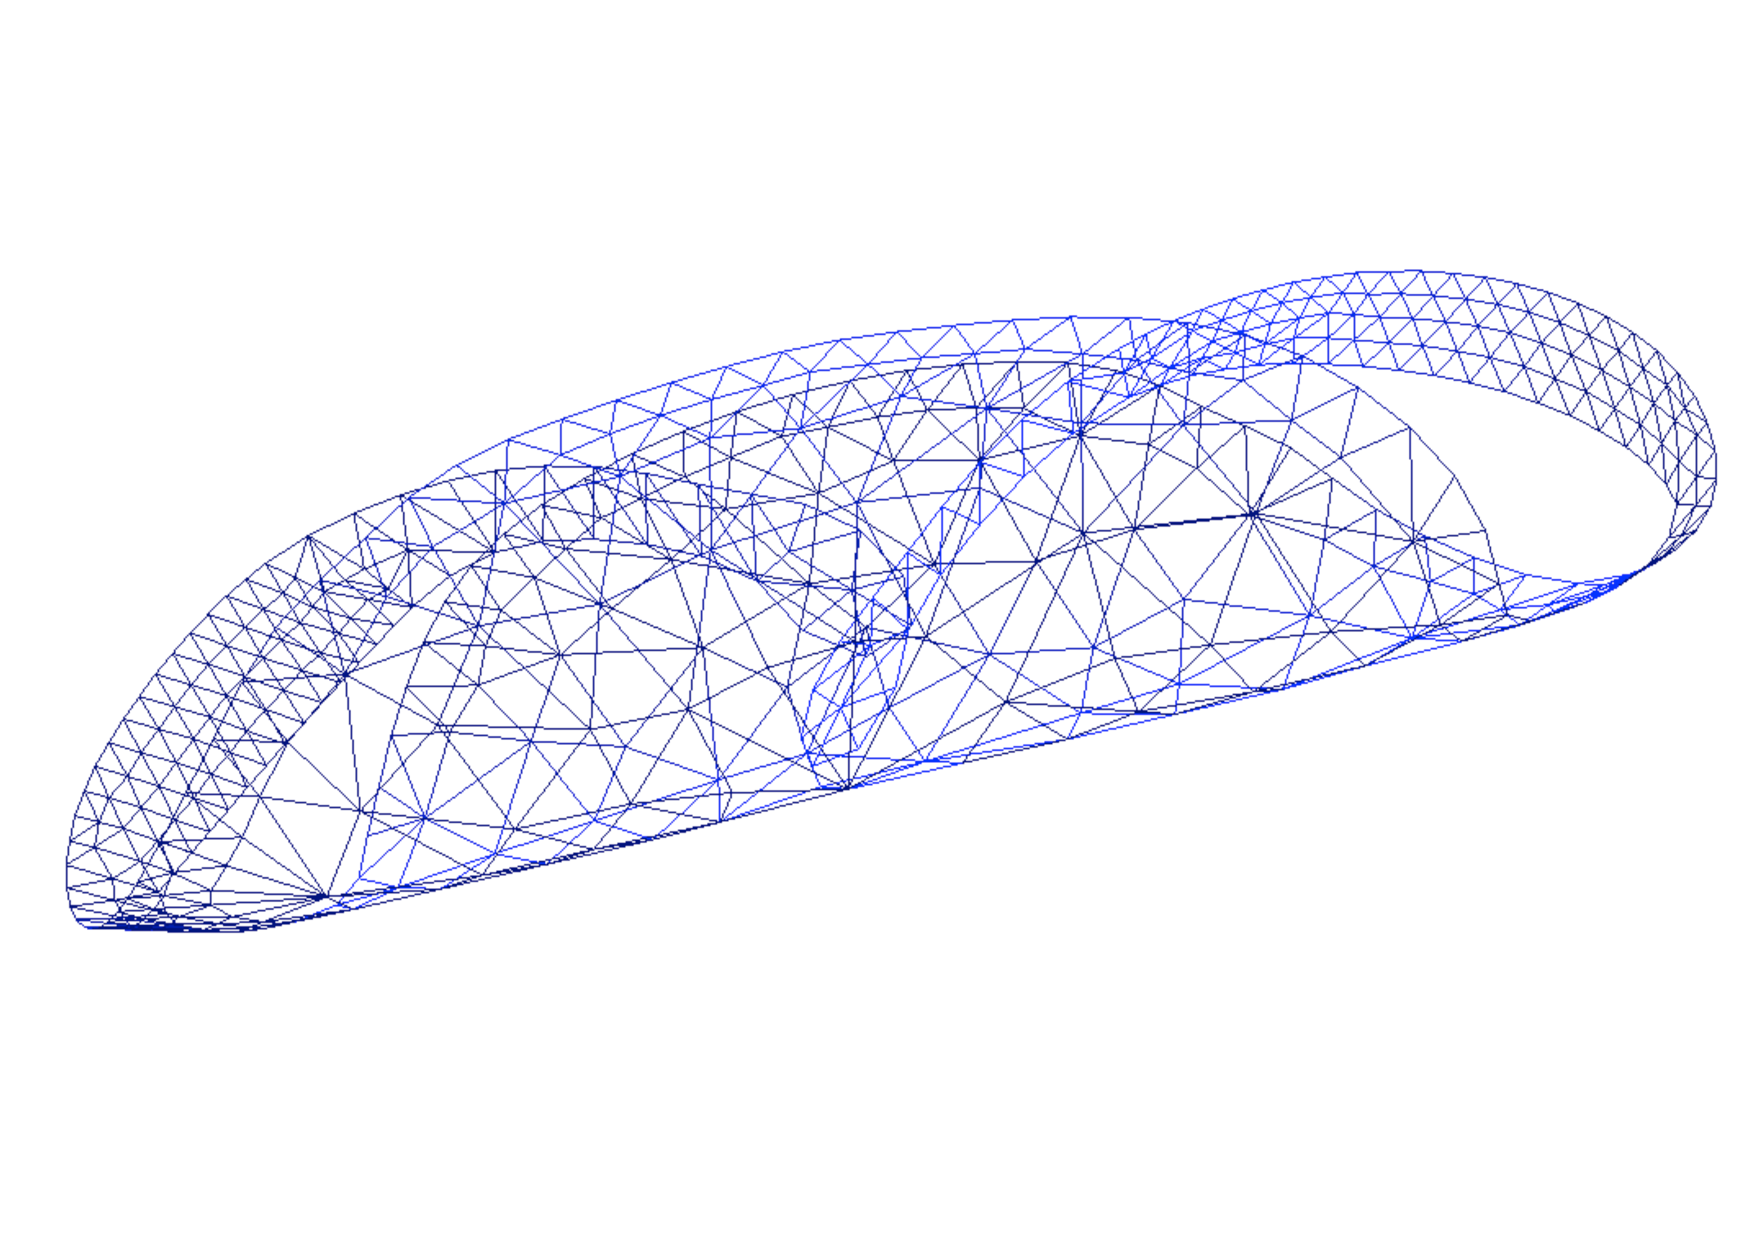
\includegraphics[width=7cm]{chapter9/implant_folding4.pdf}
\caption [Folding of intra-ocular implant] {Top: intermediary steps of the intra-ocular implant folding. Bottom: fully folded implant ready to be placed into the injection device.}
\label{chap9:fig-implantFolding}
\end{figure}

Results of our simulation are illustrated in \fig{chap9:fig-simu-results}. We can notice the progressive deployment of the implant when it exits the injector.  The shape of the intra-ocular lens remains very close to that of a real one during all stages of the simulation: within the injector, during the ejection phase, and when in place within the capsule. Due to the high stiffness and low mass of the lens, a direct sparse solver was used at each time step (dt $= 0.01$\,s) rather than an iterative solver, resulting in a more accurate and more stable simulation, to the detriment of computation times (about 5 FPS for the complete simulation, and about 10 FPS for the deformation only, on a 2.4 GHz processor).

% Link where images from surgery have been found: http://asianophthalmology.org/articles/?a=articles&p=6
\begin{figure}[!h]
\centering
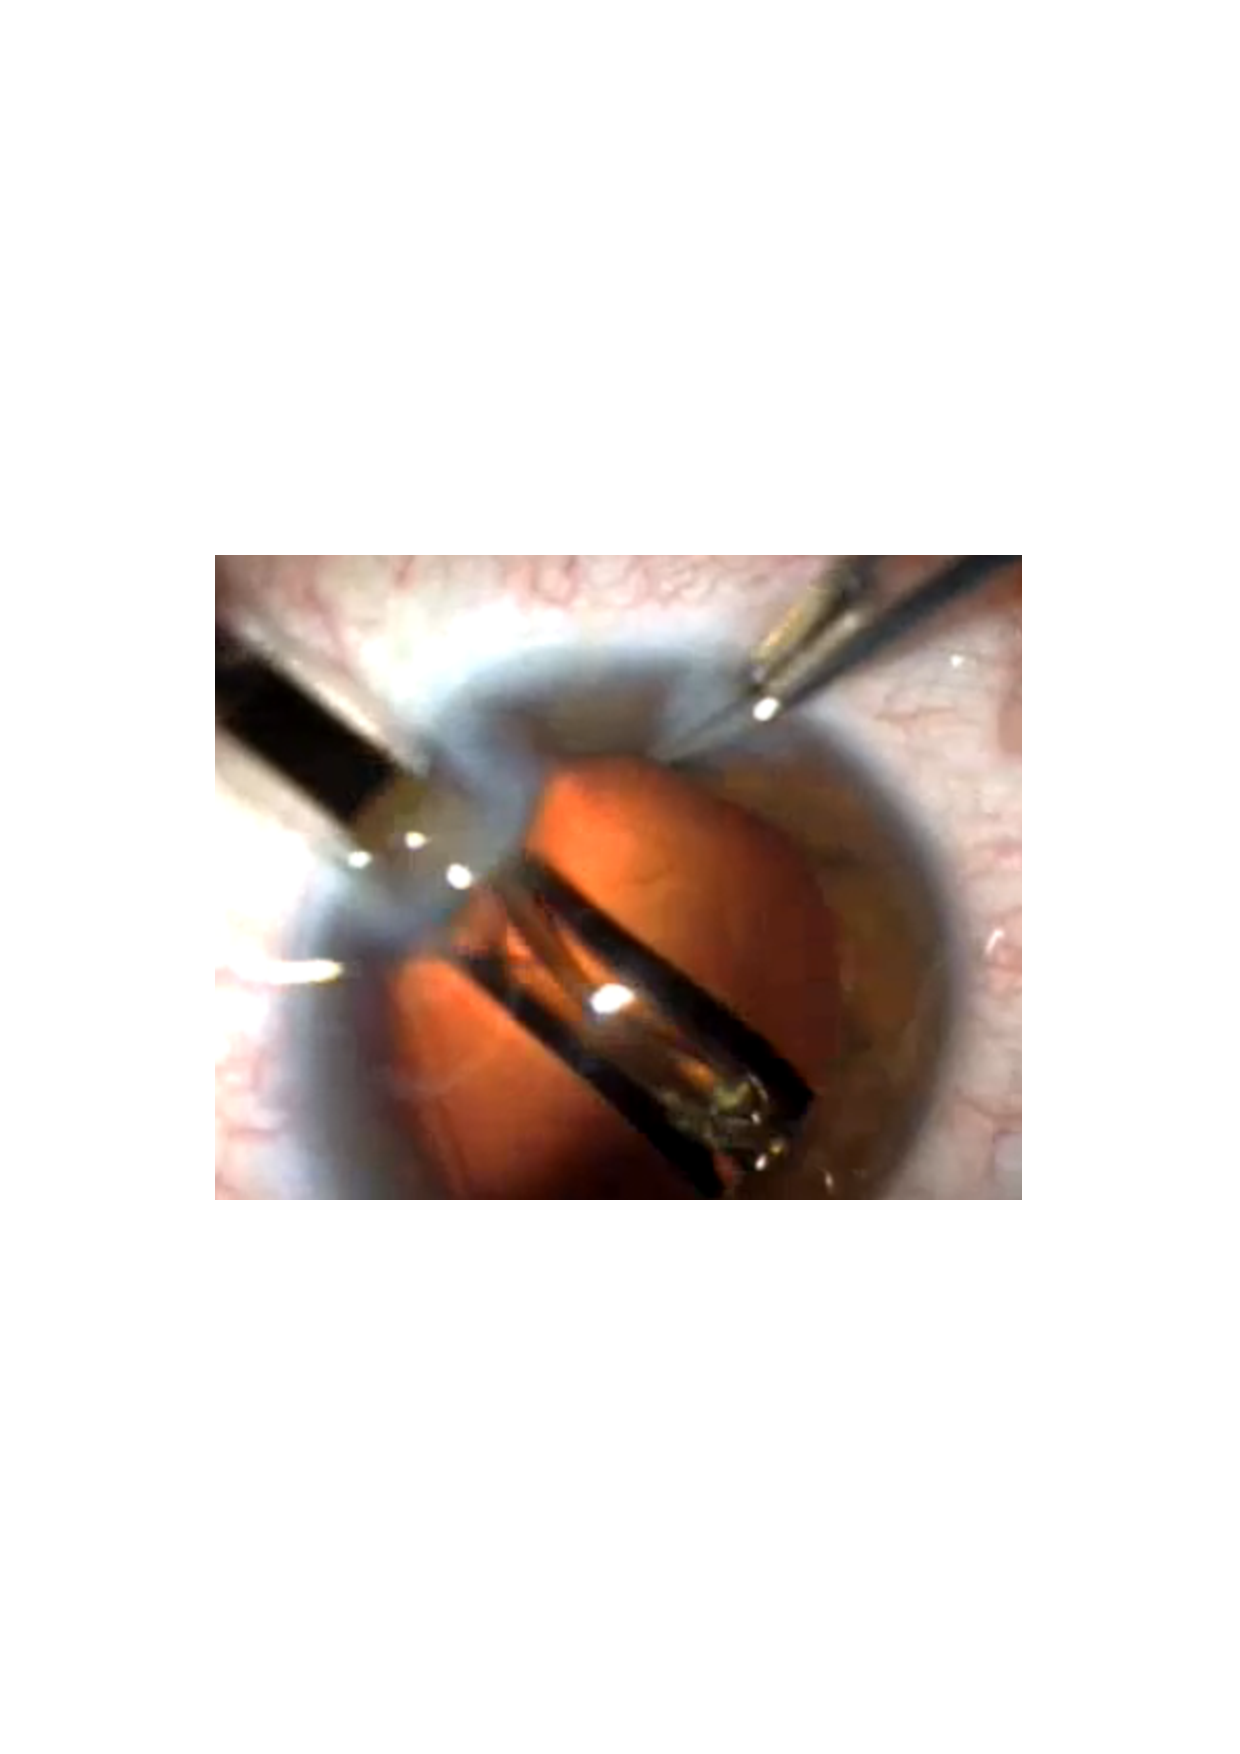
\includegraphics[width=4.5cm]{chapter9/surgery1.pdf}
\hfill
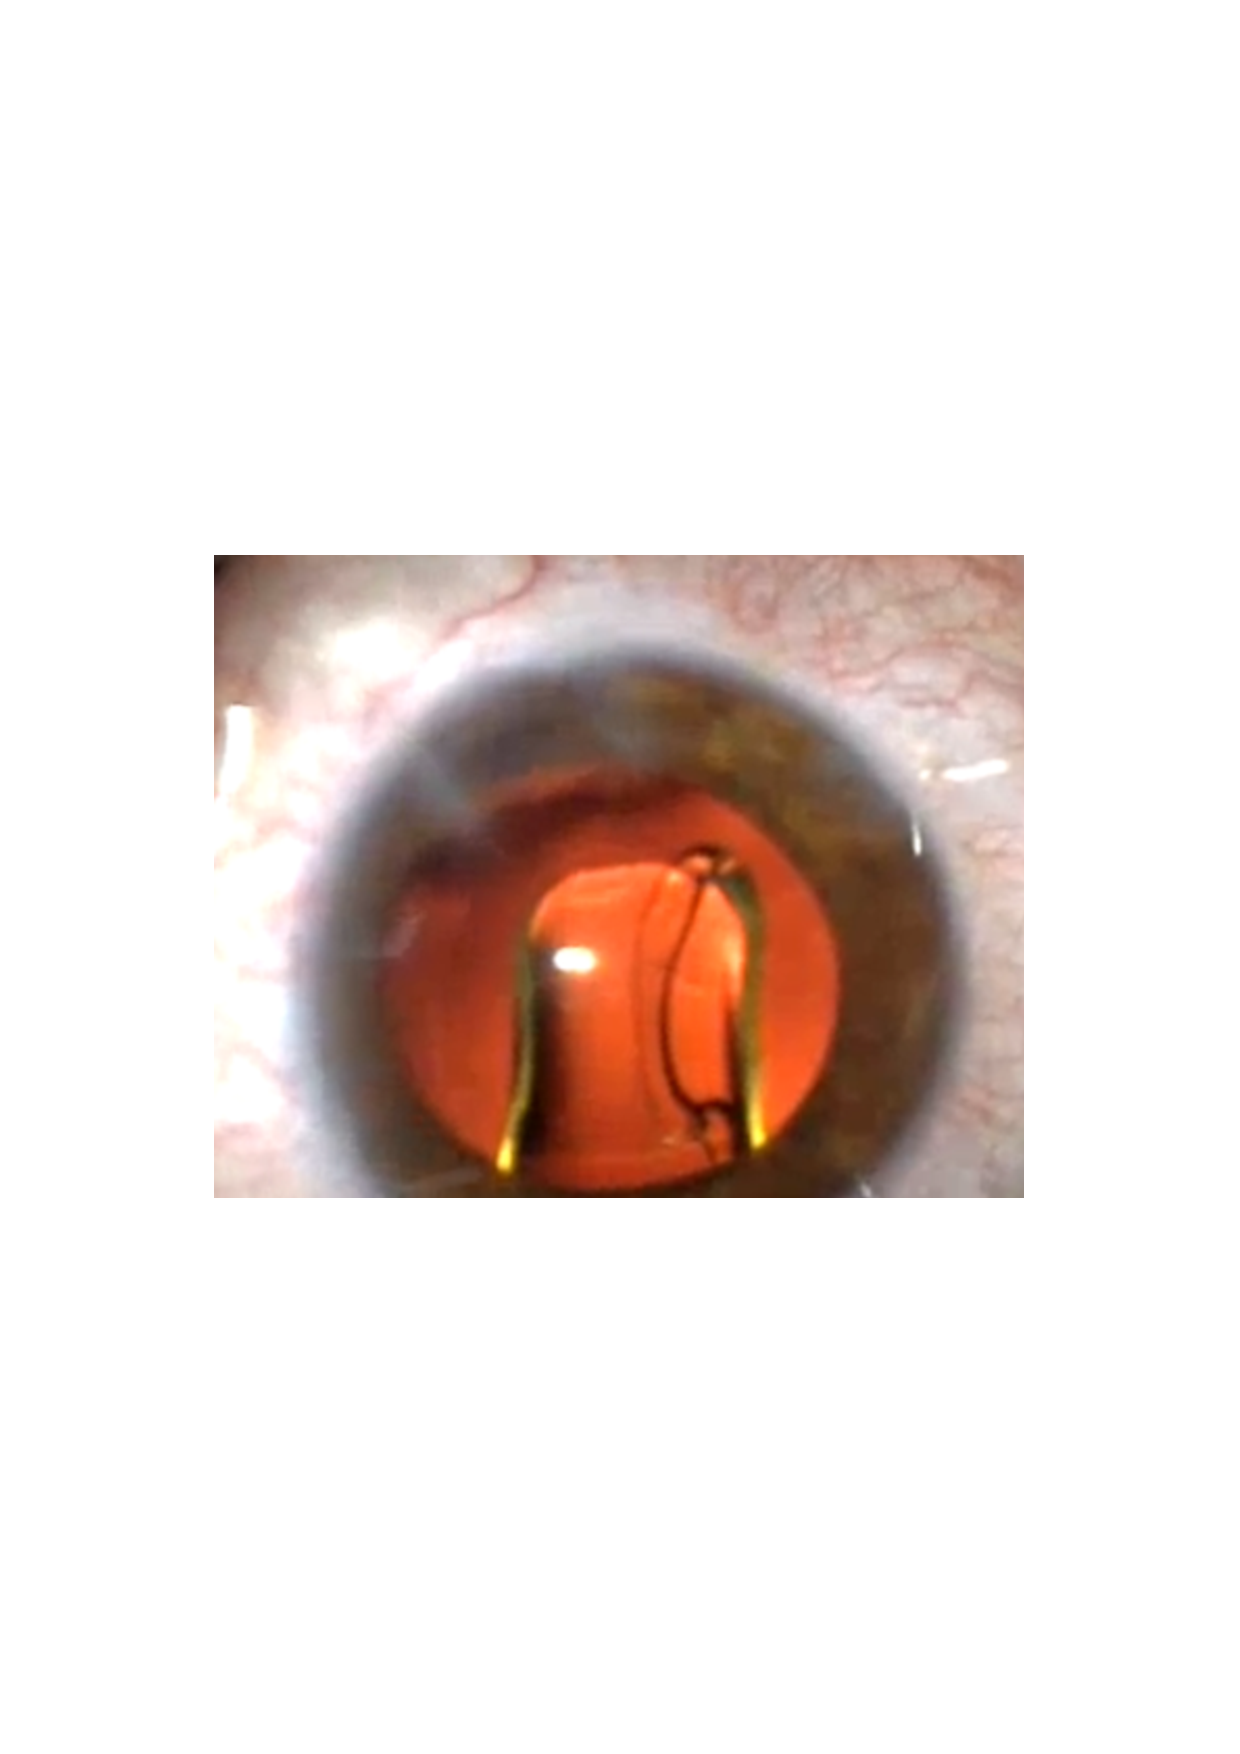
\includegraphics[width=4.5cm]{chapter9/surgery2.pdf}
\hfill
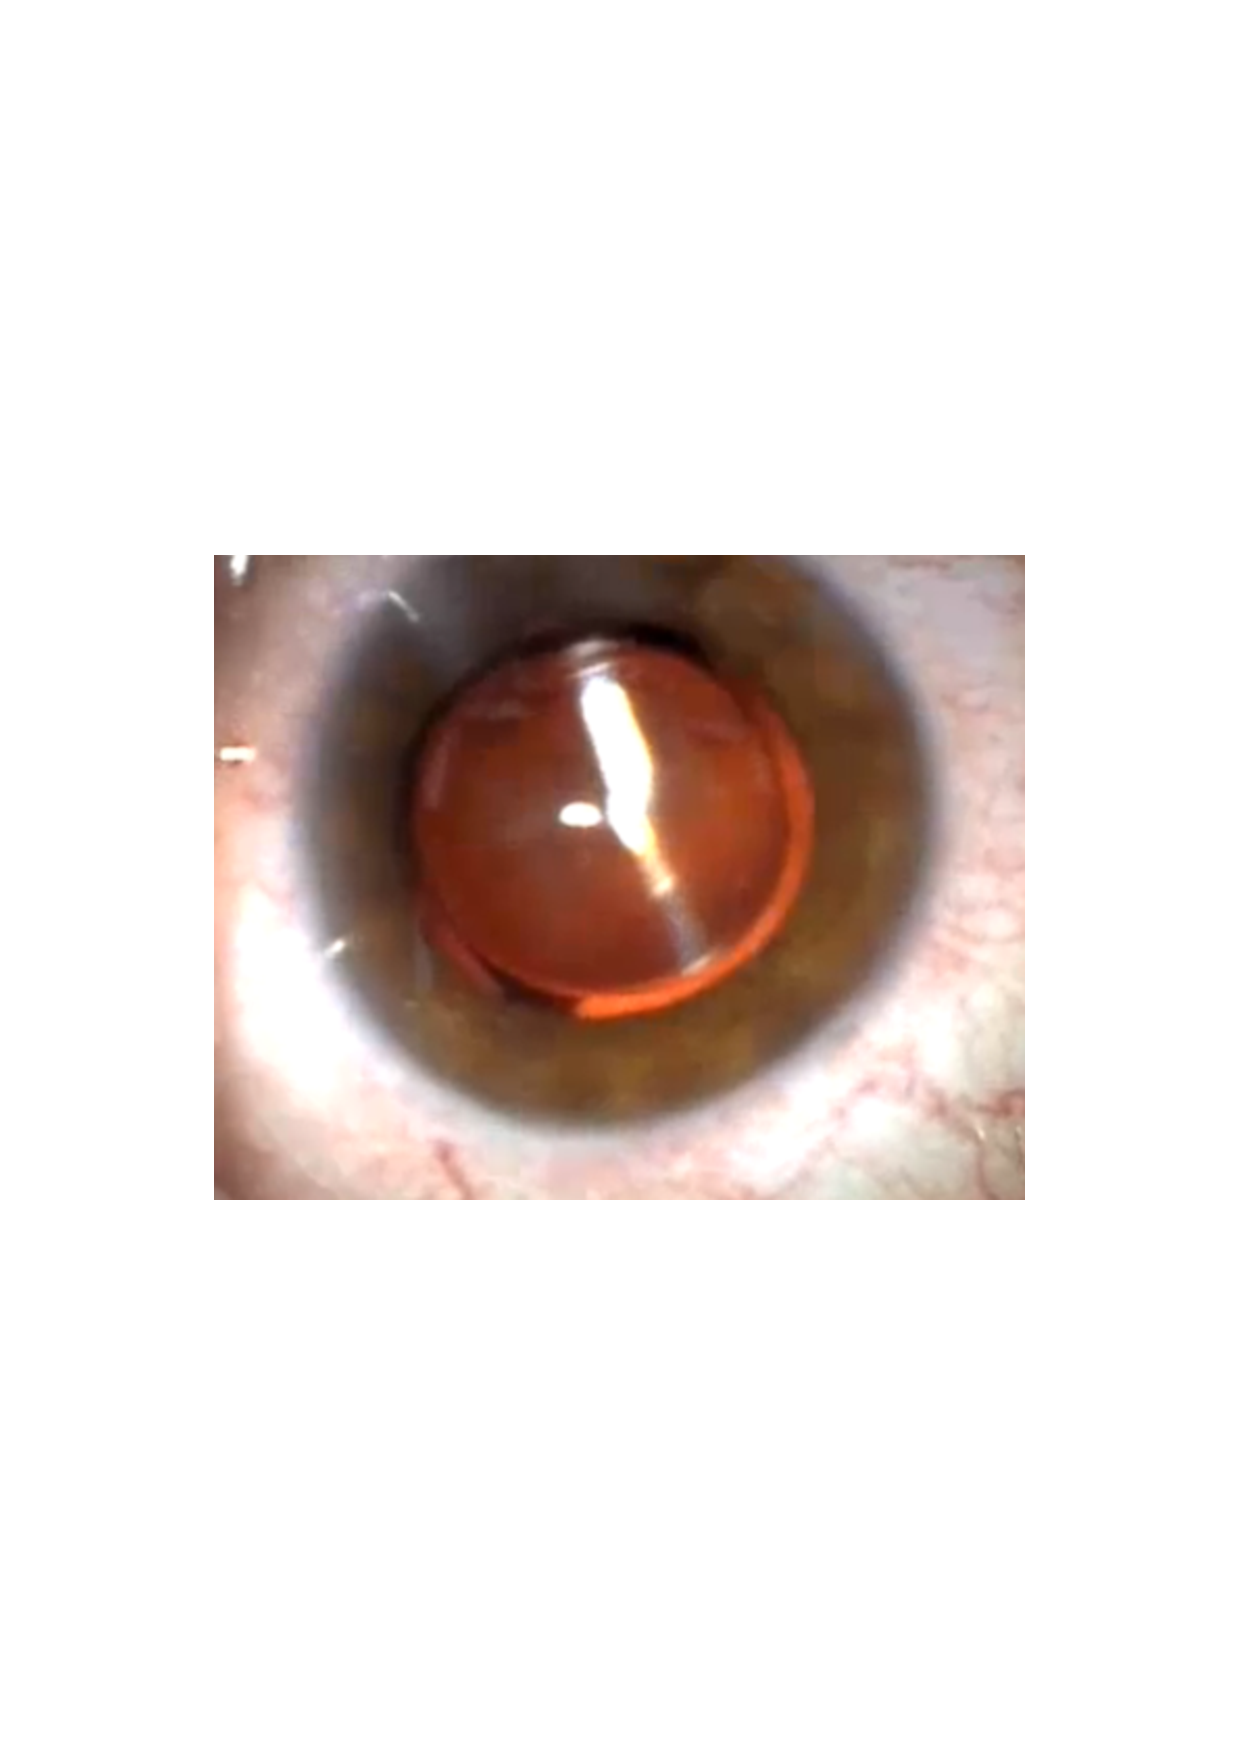
\includegraphics[width=4.5cm]{chapter9/surgery3.pdf} \\
\vspace{0.1cm}
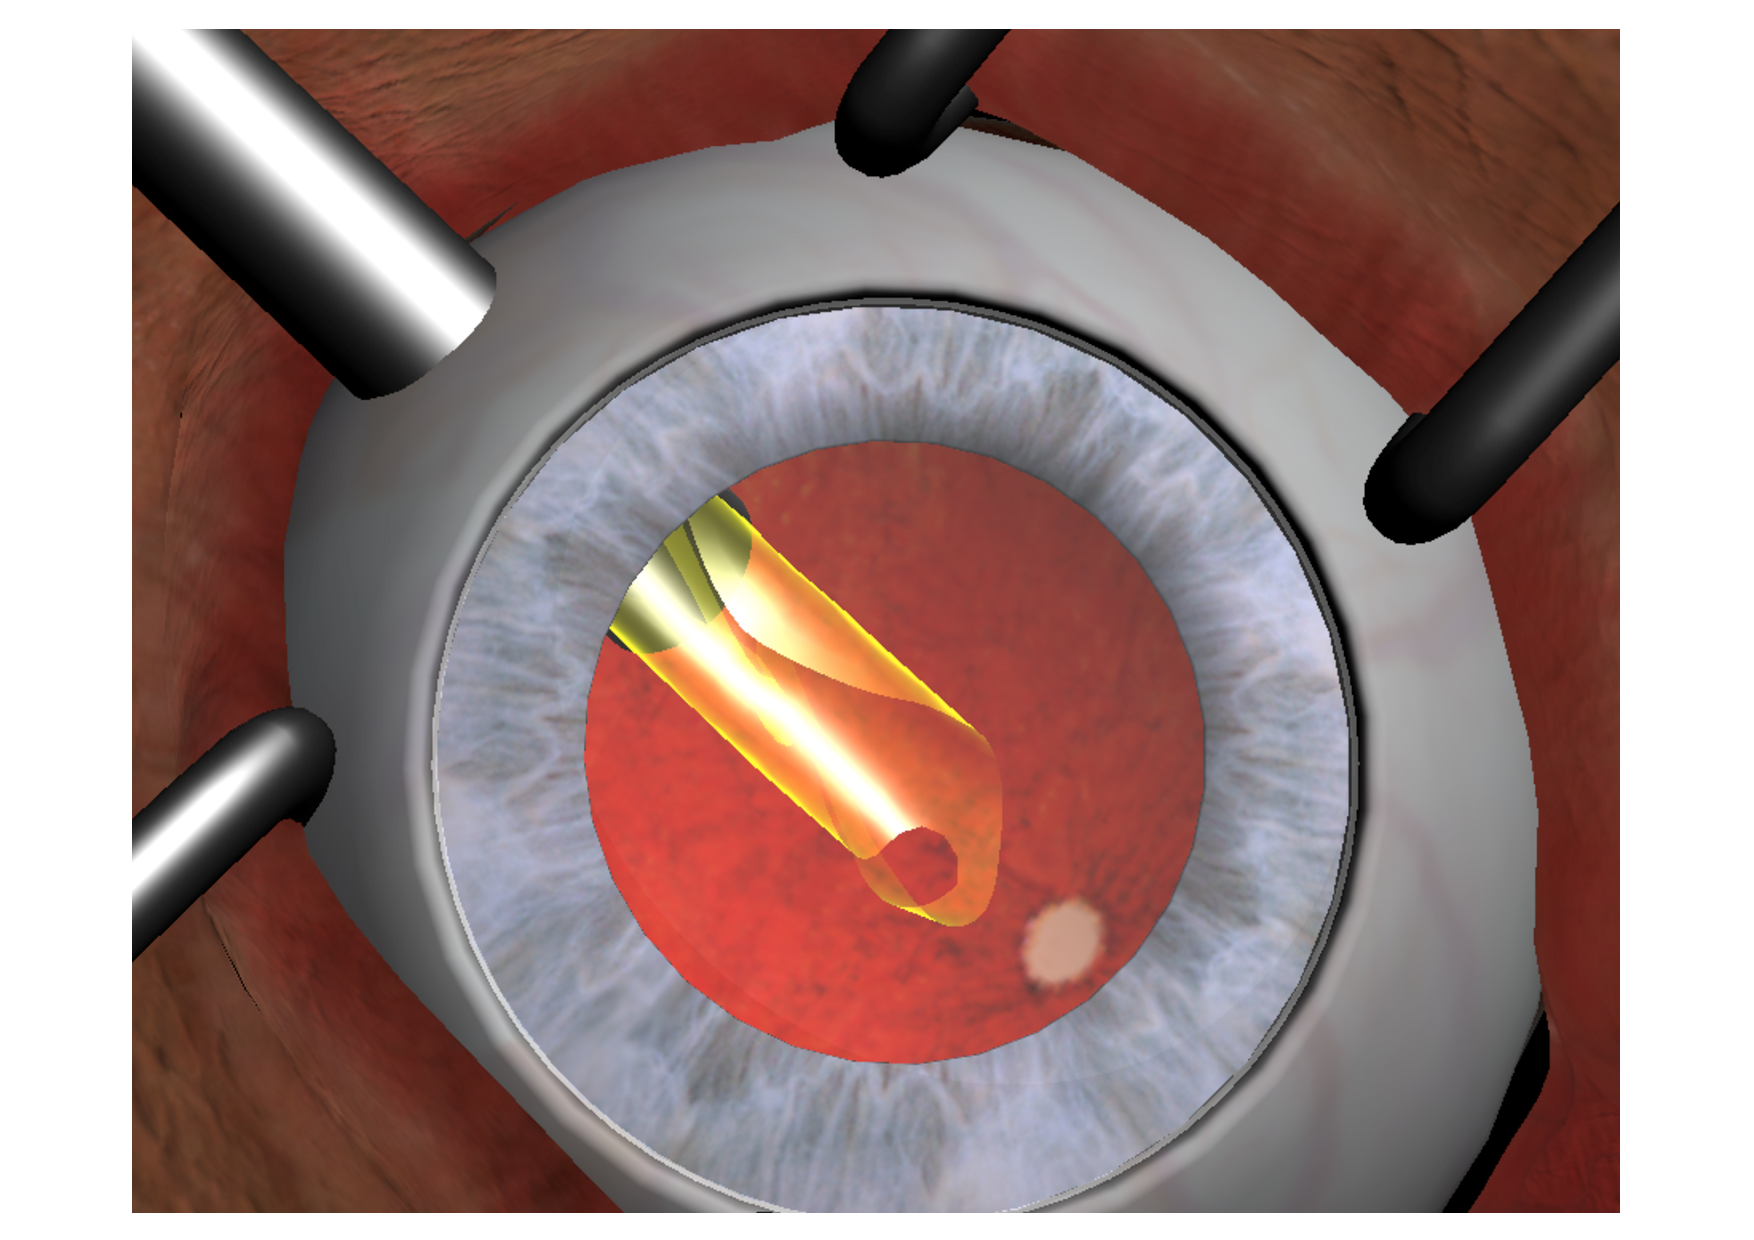
\includegraphics[width=4.5cm]{chapter9/simu1.pdf}
\hfill
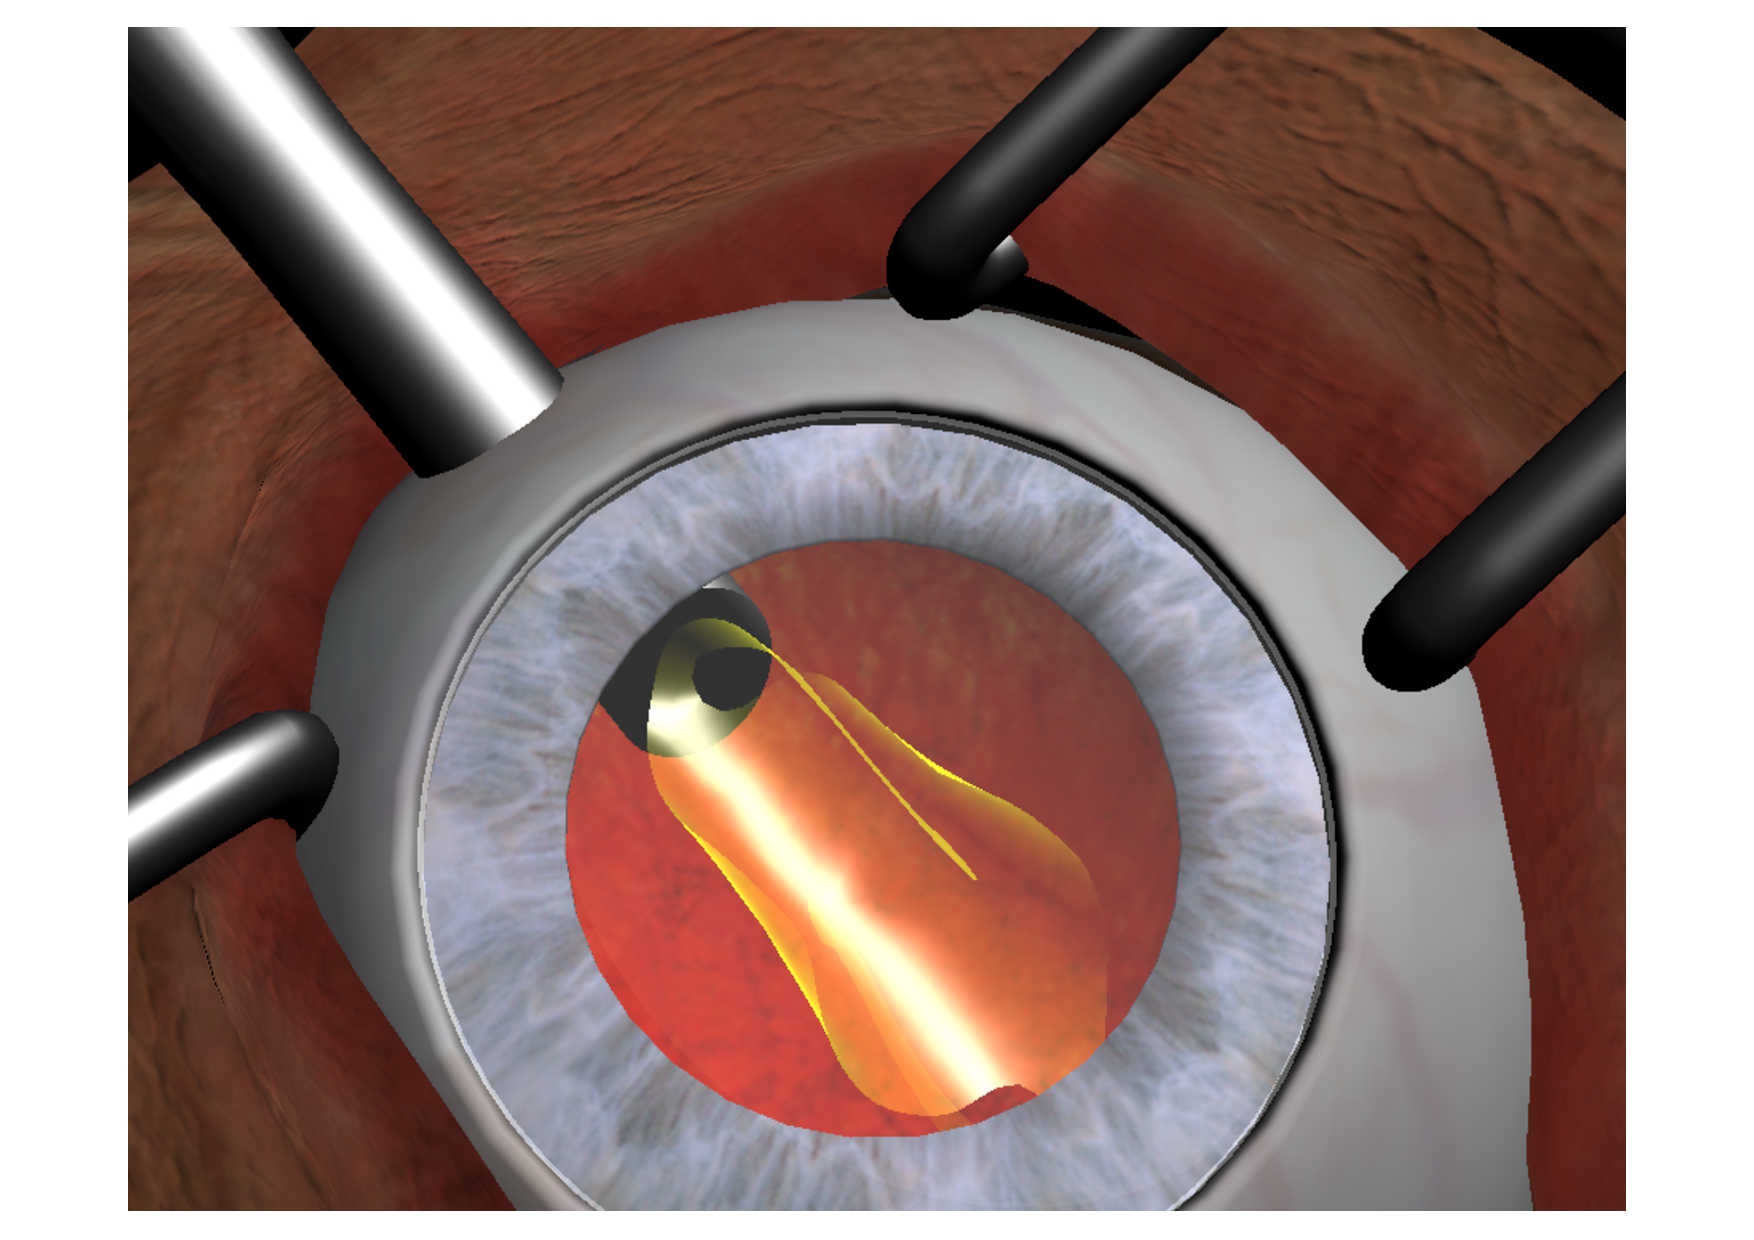
\includegraphics[width=4.5cm]{chapter9/simu2.pdf}
\hfill
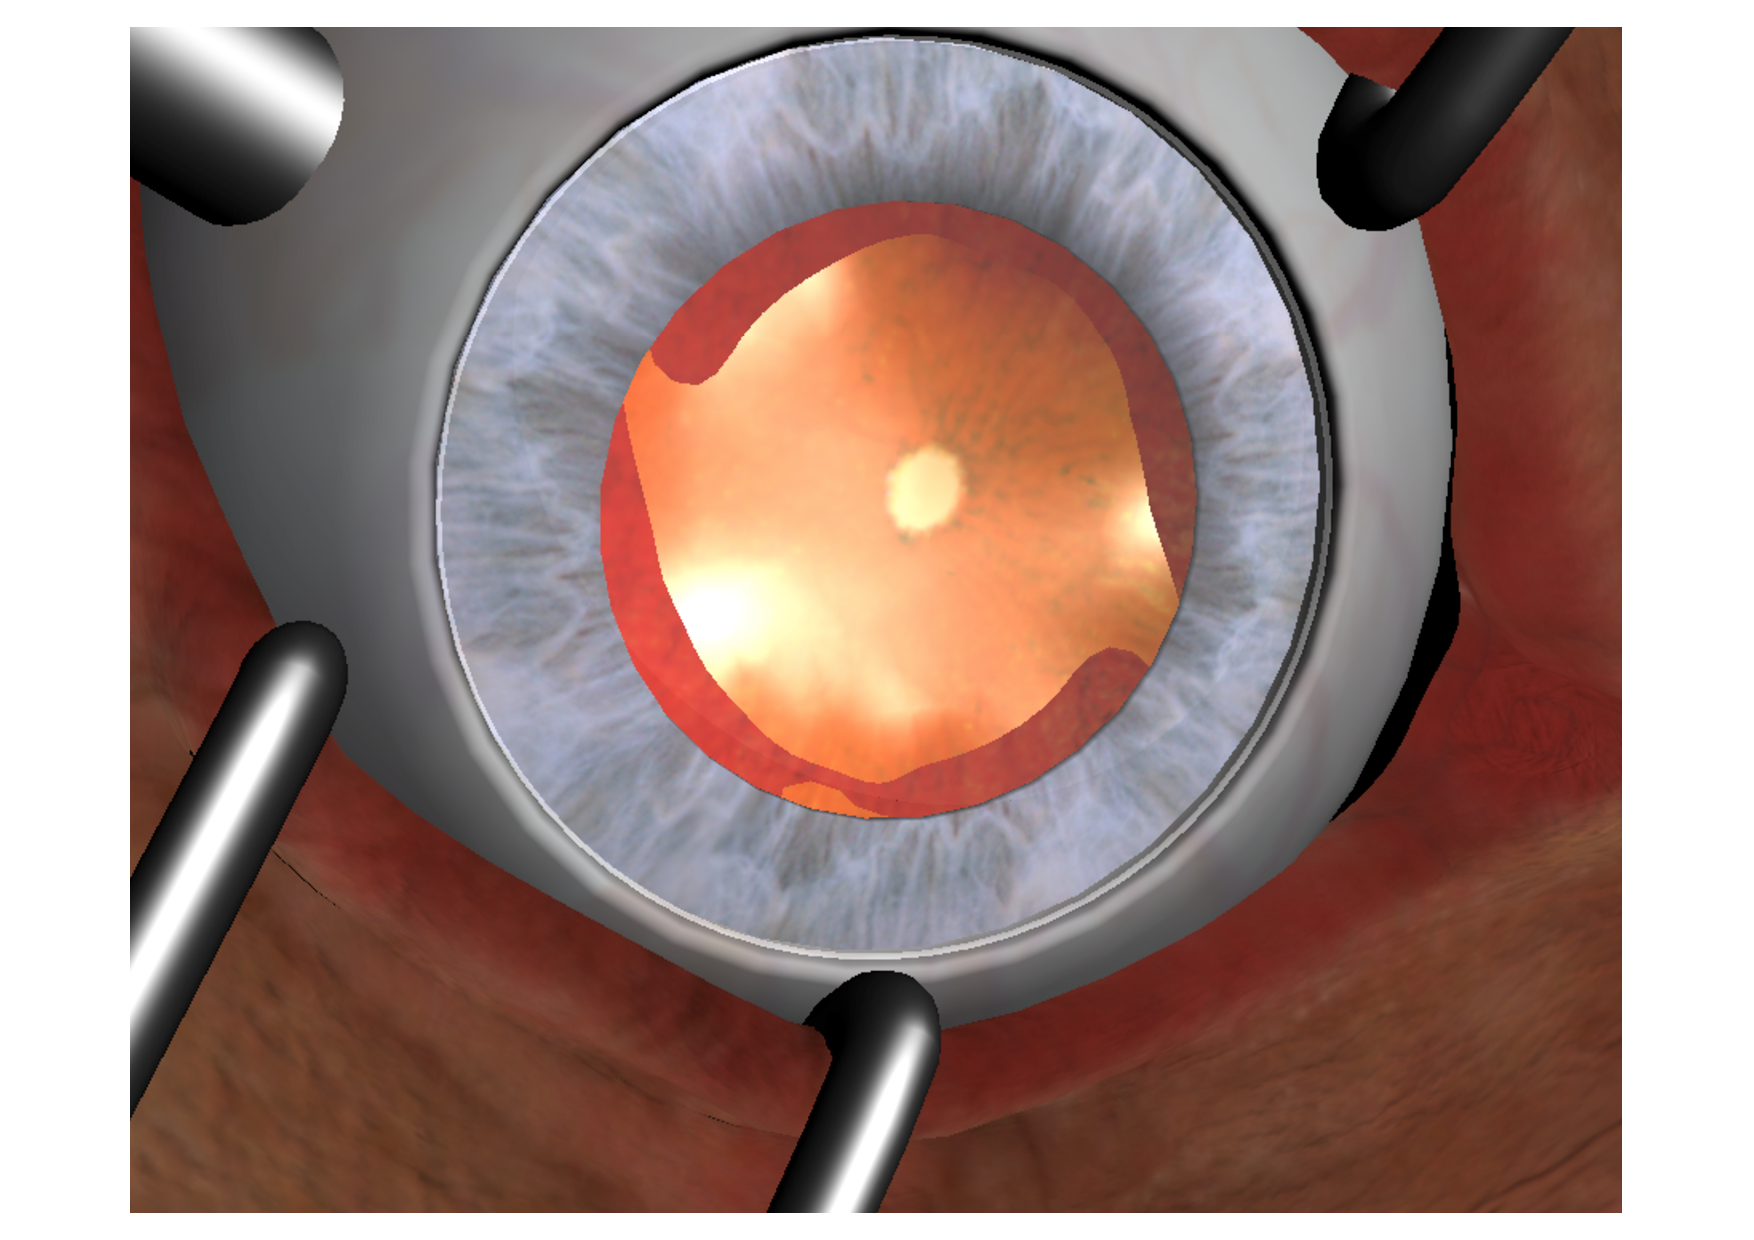
\includegraphics[width=4.5cm]{chapter9/simu3.pdf}
\caption [Lens imlant] {Three steps of the simulation of the intra-ocular lens implant injection and its deployment within the lens capsule. Top: images from a real cataract surgery, courtesy of Dr. Tarek Youssef, ophtalmologist in Canada. Below: our simulation of the implant's deployment.}
\label{chap9:fig-simu-results}
\end{figure}

		
\section{Discussion}

We proposed a co-rotational formulation for shell elements by extending a classical in-plane triangular finite element approach. This simple shell element can efficiently handle both membrane, bending and twist forces. The validity of our approach has been demonstrated though comparison with theoretical results. It was then applied it to a rather complex application: the simulation of intra-ocular lens implant deployment in a cataract surgery simulation. These preliminary results are very encouraging and show the potential of such models. Examples include the modelling of hollow anatomical structures (stomach, colon, etc.), the simulation of cardiac valve leaflets, and blood vessels. However, to model the deformation of complex anatomical structures using shell elements, the first step is to describe its surface with curved patches. In the next section, we propose to study how to approximate the surface of anatomical structures with shell elements.
